\documentclass[12pt,a4paper,twoside]{book}
\usepackage{titlesec}
% Κάνει το Chapter να μοιάζει με Section
\titleformat{\chapter}[hang]
{\normalfont\Large\bfseries}{\thechapter.}{1em}{}
\titlespacing*{\chapter}{0pt}{-20pt}{20pt} % Μειώνει και το κενό πάνω από τον τίτλο
% Language setup for Greek and English
\usepackage[english,greek]{babel}
\usepackage[utf8]{inputenc}
\usepackage[T1,LGR]{fontenc}
% Font setup
\usepackage{fontspec}
\setmainfont{Linux Libertine O}[Scale=0.9]
\setsansfont{Linux Biolinum}[Scale=0.9]
\setmonofont{DejaVu Sans Mono}[Scale=0.9]
% Other necessary packages
\usepackage{enumitem}
\usepackage{graphicx}
\usepackage{amsmath}
\usepackage{makeidx}
\usepackage{multicol}
\usepackage{multirow}
\usepackage{hanging}
\usepackage{adjustbox}
\usepackage{amssymb}
\usepackage{stackengine}
\usepackage{ifthen}
\usepackage{array}
\usepackage{tcolorbox}
\tcbuselibrary{skins,breakable}
\usepackage{minted}
\usepackage{listings}
\usepackage{indentfirst}
\usepackage{float}
\usepackage{subcaption}
\usepackage{xcolor}
\usepackage{cancel}
\usepackage{pdfpages}

% Bibliography setup
\usepackage[numbers,square,sort\&compress,longnamesfirst]{natbib}
\bibliographystyle{hellas}
\makeatletter

% Use this for a chapter that should not force a new page.
\newcommand{\chapteronsamepage}[1]{%
    \begingroup
    \let\clearpage\relax
    \let\cleardoublepage\relax
    \par\vspace{\baselineskip}%
    \chapter{#1}%
    \endgroup
}
\makeatother

% Define commands for authoryear-style citations
\newcommand{\citeauthyear}[1]{[\citeauthor{#1} \citeyear{#1}]}
\newcommand{\Citeauthyear}[1]{\Citeauthor{#1} [\citeyear{#1}]}

\makeatletter
\renewenvironment{thebibliography}[1]%
     {\@mkboth{\MakeUppercase\refname}{\MakeUppercase\refname}%
      \list{\@biblabel{\@arabic\c@enumiv}}%
           {\settowidth\labelwidth{\@biblabel{#1}}%
            \leftmargin\labelwidth%
            \advance\leftmargin\labelsep%chktex 41
            \@openbib@code%
            \usecounter{enumiv}%
            \let\p@enumiv\@empty%chktex 21
            \renewcommand\theenumiv{\@arabic\c@enumiv}}%
      \sloppy%
      \clubpenalty4000%
      \@clubpenalty\clubpenalty%
      \widowpenalty4000%
      \sfcode`\.\@m}%chktex 21
     {\def\@noitemerr%chktex 21
        {\@latex@warning{Empty `thebibliography' environment}}%
      \endlist}
\makeatother
% Page & text layout
\usepackage{geometry}
\geometry{
   a4paper,
   top=2.5cm,
   bottom=2.5cm,
   left=2.5cm,
   right=2.5cm
}
% Headers & footers
\usepackage{fancyhdr}
\pagestyle{fancyplain}
\fancyhf{} % Clear all header/footer fields

% Define plain style for chapter pages and TOC
\fancypagestyle{plain}{%
    \fancyhf{} % Clear all header/footer fields
    \renewcommand{\headrulewidth}{0pt} % Remove header rule
    \renewcommand{\footrulewidth}{0pt} % Remove footer rule
}

% Define TOC style with specific headers
\fancypagestyle{tocstyle}{%
    \fancyhf{} % Clear all header/footer fields
    \fancyhead[LE]{\thepage}
    \fancyhead[CE]{\leftmark}
    \fancyhead[CO]{\rightmark}
    \fancyhead[RO]{\thepage}
    \renewcommand{\headrulewidth}{0pt}
}

% Fix marks to prevent premature updates - use extramarks to delay mark updates
\renewcommand{\sectionmark}[1]{\markboth{#1}{}}
\renewcommand{\subsectionmark}[1]{\markright{#1}}

% Redefine \tableofcontents to use tocstyle
\let\oldtableofcontents\tableofcontents
\renewcommand{\tableofcontents}{%
    \clearpage
    % First page of TOC should be empty
    \thispagestyle{empty}
    \pagestyle{tocstyle}
    \oldtableofcontents % chktex 1
    \clearpage
    \pagestyle{fancy}
    % Regular pages header settings
    \fancyhead[LE]{\thepage} % Left header on Even pages: Shows page number
    \fancyhead[CE]{\leftmark} % Center header on Even pages: Shows chapter name (stored in \leftmark)
    \fancyhead[RE]{ΚΕΦ. \thechapter} % Right header on Even pages: Shows "ΚΕΦ." followed by chapter number % chktex 12

    \fancyhead[LO]{\thesection} % Left header on Odd pages: Shows current section number
    \fancyhead[CO]{\rightmark} % Center header on Odd pages: Shows section name (stored in \rightmark)
    \fancyhead[RO]{\thepage} % Right header on Odd pages: Shows page number

    \renewcommand{\headrulewidth}{0.4pt} % Sets thickness of the horizontal line below the header

    % Redefine chapter mark to remove "Chapter" prefix
    \renewcommand{\chaptermark}[1]{\markboth{##1}{}}
    % Redefine section mark to delay updates until after page break
    % This prevents showing the next section number when current section ends at page bottom
    \renewcommand{\sectionmark}[1]{%
        \markright{##1}%
    }
    \renewcommand{\subsectionmark}[1]{}
}

% Additional fix: Make section marks update at first mark instead of both marks
\makeatletter
\renewcommand\sectionmark[1]{%
  \markright{%
    \ifnum \c@secnumdepth >\z@
      \thesection\quad
    \fi
    #1}}
\makeatother

% Make table of contents use plain style
\addtocontents{toc}{\protect\thispagestyle{plain}}

% Hyperlinks
\usepackage{hyperref}
\usepackage{bookmark}                                       % Add this line to fix the hyperref warnings
\hypersetup{
    colorlinks=true,
    linkcolor=blue,
    citecolor=blue,
    filecolor=blue,
    urlcolor=customCodeBlue,
    unicode,
    pdftitle={BeautyHub}, % chktex 19
    pdfsubject={Αναφορά Εργασίας},
    pdfborderstyle={/S/U/W 1},                              % Underline links
}
\usepackage{tikz}
\usetikzlibrary{positioning, shapes.geometric, arrows.meta}
\usepackage{pgfplots}
\pgfplotsset{compat=1.18}
\usetikzlibrary{calc,arrows.meta,positioning}

\definecolor{customRed}{HTML}{FF5F5A}                       % using hexadecimal
\definecolor{customYellow}{HTML}{FFBE2E}                    % using hexadecimal
\definecolor{customGreen}{HTML}{2ACA44}                     % using hexadecimal
\definecolor{customPurple}{HTML}{C477DB}                    % using hexadecimal
\definecolor{customBlue}{HTML}{052538}                      % using hexadecimal
\definecolor{customLightBlue}{HTML}{60ADEC}                 % using hexadecimal
\definecolor{customGray}{HTML}{A0A0A0}                      % using hexadecimal
\definecolor{customBlack}{HTML}{000000}                     % using hexadecimal

% Define a lighter gray for background and darker colors for text
\definecolor{customBgGray}{HTML}{E0E0E0}         % Light gray background
\definecolor{customCodeRed}{HTML}{C92A2A}        % Darker red
\definecolor{customCodeYellow}{HTML}{E67700}     % Darker yellow/orange
\definecolor{customCodeGreen}{HTML}{087F23}      % Darker green
\definecolor{customCodePurple}{HTML}{7B1FA2}     % Darker purple
\definecolor{customCodeBlue}{HTML}{1976D2}       % Darker blue
\definecolor{customCodeBlack}{HTML}{1A1A1A}      % Lighter black

% Custom commands for language switching
\newcommand{\en}[1]{\foreignlanguage{english}{#1}}
\newcommand{\gr}[1]{\foreignlanguage{greek}{#1}}
% Custom command for coloring
\newcommand{\blue}[1]{\textcolor{blue}{#1}}
% Index
\makeindex
% Set headheight to avoid fancyhdr warnings
\setlength{\headheight}{14.5pt}

% Adjust chapter spacing
%\titleformat{\chapter}[display]
%{\normalfont\huge\bfseries}{\chaptertitlename\ \thechapter}{15pt}{\Huge}
%\titlespacing*{\chapter}{0pt}{-10pt}{20pt}

% Adjust section spacing
\titlespacing*{\section}{0pt}{10pt}{10pt}

% Use first-line paragraph indentation instead of blank line spacing
\setlength{\parindent}{1.5em}
\setlength{\parskip}{0pt}

% Make figure placement less strict
\setcounter{topnumber}{2}
\setcounter{bottomnumber}{2}
\setcounter{totalnumber}{4}
\renewcommand{\topfraction}{0.85}
\renewcommand{\bottomfraction}{0.85}
\renewcommand{\textfraction}{0.15}
\renewcommand{\floatpagefraction}{0.7}

\begin{document}
% Start Arabic numbering from the beginning but hide numbers
\pagenumbering{arabic}
% Add this command to prevent blank pages
\let\cleardoublepage\clearpage

% Set main language to Greek
\selectlanguage{greek}

% Title page with hidden number
\begin{titlepage}
    \begin{center}
        % University logo and information
        \vspace*{3.5cm}
        \begin{minipage}[c]{0.38\textwidth}
            \centering
            
\includegraphics[width=6.0cm]{logo.png}
        \end{minipage}
 

        {\large Τεχνολογία Λογισμικού }\\[3cm]

        \vspace*{\fill}
 
        \begin{tabular}{l l l}
            \large Εμμανουήλ Τσιόρβας & \large 1072622 & \large up1072622@ac.upatras.gr \\
            \large Αθανάσιος Γαβριήλ & \large 1093335 & \large up1093335@ac.upatras.gr \\
            \large Κωνσταντίνα - Μαρία Δεδεμάδη & \large 1093350 & \large up1093350@ac.upatras.gr \\
            \large Γεώργιος Καπατσούλιας & \large 1093377 & \large up1093377@ac.upatras.gr \\
            \large Αντώνιος Τσιπουλάκος & \large 1097450 & \large up1097450@ac.upatras.gr \\

        \end{tabular}\\[3.0cm]

        {\normalsize Πάτρα, 2026}
    \end{center}
    \thispagestyle{empty}
\end{titlepage}

\tableofcontents

\chapter{Project-description-v0.1}
\section{Περιγραφή Εργασίας}
Αντικείμενο της παρούσας εργασίας αποτελεί η υλοποίηση της πλατφόρμας BeautyHub, ενός ολοκληρωμένου πληροφοριακού συστήματος που στοχεύει στην αυτοματοποίηση των διαδικασιών ενός σύγχρονου κομμωτηρίου. Η εφαρμογή λειτουργεί ως ένας κεντρικός κόμβος που συνδέει αρμονικά τη διοίκηση της επιχείρησης, το προσωπικό και την πελατεία, εξαλείφοντας τις παραδοσιακές δυσκολίες του προγραμματισμού και της επικοινωνίας. Μέσω ενός φιλικού προς τον χρήστη περιβάλλοντος, το BeautyHub μετατρέπει τη διαδικασία της κράτησης από μια χρονοβόρα τηλεφωνική συνεννόηση σε μια απλή και γρήγορη ψηφιακή εμπειρία.

Η καρδιά του BeautyHub είναι το έξυπνο σύστημα κρατήσεων. Οι πελάτες μπορούν να κλείνουν το ραντεβού τους online, επιλέγοντας τον hair expert της προτίμησής τους και την υπηρεσία που επιθυμούν, ενώ το σύστημα αποστέλλει αυτόματες υπενθυμίσεις για την αποφυγή ακυρώσεων. Κάθε πελάτης διατηρεί το προσωπικό του προφίλ, όπου αποθηκεύεται το ιστορικό των επισκέψεών του και οι προτιμήσεις του.

Το BeautyHub εισάγει ένα προηγμένο σύστημα ελέγχου αποθεμάτων. Η εφαρμογή παρακολουθεί σε πραγματικό χρόνο τη χρήση αναλώσιμων (βαφές, οξυζενέ, σαμπουάν) και ειδοποιεί αυτόματα για ελλείψεις. Παράλληλα, η πλατφόρμα περιλαμβάνει ένα πλήρως λειτουργικό ηλεκτρονικό κατάστημα, επιτρέποντας στους πελάτες να αγοράζουν τα αγαπημένα τους επαγγελματικά προϊόντα περιποίησης απευθείας μέσα από την εφαρμογή. Το ηλεκτρονικό κατάστημα συνδέεται αυτόματα με το σύστημα της αποθήκης, διασφαλίζοντας ότι η διαθεσιμότητα των προϊόντων είναι πάντα ενημερωμένη, ενώ προσφέρει τη δυνατότητα στους πελάτες να προμηθεύονται τα προϊόντα που χρησιμοποίησε ο κομμωτής τους κατά τη διάρκεια της επίσκεψής τους.

Η πλατφόρμα ενσωματώνει έναν μηχανισμό αξιολόγησης δύο επιπέδων, προσφέροντας απόλυτη διαφάνεια στην ποιότητα των υπηρεσιών. Μετά από κάθε ραντεβού, οι πελάτες έχουν τη δυνατότητα να βαθμολογήσουν τόσο τη συνολική εμπειρία τους στο κομμωτήριο (χώρος, εξυπηρέτηση, καθαριότητα), όσο και τον hair expert που τους ανέλαβε (τεχνική κατάρτιση, επικοινωνία, αποτέλεσμα). Τα δεδομένα αυτά τροφοδοτούν ένα δυναμικό σύστημα analytics, το οποίο παράγει αναλυτικά στατιστικά απόδοσης. Οι ιδιοκτήτες μπορούν έτσι να εντοπίζουν τους πιο δημοφιλείς υπαλλήλους, να παρακολουθούν το επίπεδο ικανοποίησης του κοινού σε πραγματικό χρόνο και να λαμβάνουν στρατηγικές αποφάσεις για την εκπαίδευση του προσωπικού ή την επιβράβευση των κορυφαίων συνεργατών τους.

\section{Mockup Screens}
Για την δημιουργία των παρακάτω οθονών, χρησιμοποιήθηκε το PlantUML, ένα εργαλείο ανοιχτού κώδικα που επιτρέπει τη γρήγορη δημιουργία διαγραμμάτων.

\begin{figure}[H]
    \centering
    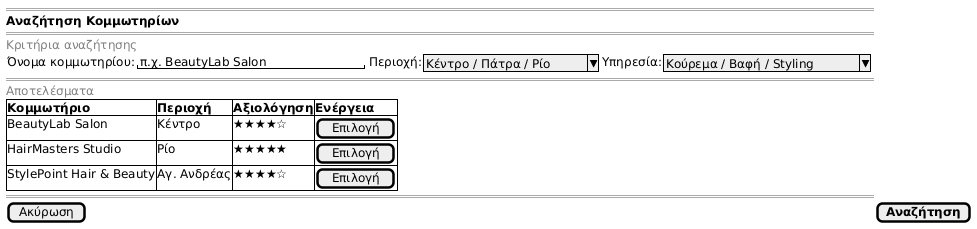
\includegraphics[width=0.8\textwidth]{mockups/αναζήτηση.png}
    \caption{Αναζήτηση και επιλογή κομμωτηρίου}
\end{figure}
\begin{figure}[H]
    \centering
    \includegraphics[width=0.8\textwidth]{mockups/προβολή ραντεβου και κλεισιμο.png}
    \caption{Αίτηση ραντεβού}
\end{figure}
\begin{figure}[H]
    \centering
    \includegraphics[width=0.8\textwidth]{mockups/τροποποιηση απο πελάτη.png}
    \caption{Αίτηση τροποποίησης ραντεβού από πελάτη}
\end{figure}
\begin{figure}[H]
    \centering
    
\includegraphics[width=0.8\textwidth]{mockups/διαχειριση ραντεβου.png}
    \caption{Διαχείριση ραντεβού από κομμωτή}
\end{figure}
\begin{figure}[H]
    \centering
    
\includegraphics[width=0.8\textwidth]{mockups/δημιουργια υπηρεσιας.png}
    \caption{Δημιουργία νέας υπηρεσίας}
\end{figure} 
\begin{figure}[H]
    \centering
    
\includegraphics[width=0.8\textwidth]{mockups/διαχειριση αποθεματος.png}
    \caption{Διαχείριση αποθεμάτων}
\end{figure}
\begin{figure}[H]
    \centering
    
\includegraphics[width=0.8\textwidth]{mockups/αξιολογηση.png}
    \caption{Αξιολόγηση υπηρεσιών και hair expert}
\end{figure}
\begin{figure}[H]
    \centering
    \includegraphics[width=0.8\textwidth]{mockups/στατιστικά.png}
    \caption{Στατιστικά κομμωτηρίου και προσωπικού}
\end{figure}

\chapter{Use-case-v0.1}
\section{Αναζήτηση Κομμωτηρίων}

\subsection{Σύντομη περιγραφή}
Ο πελάτης αναζητά κομμωτήρια με βάση την τοποθεσία, τις υπηρεσίες ή το όνομα και βλέπει τα σχετικά αποτελέσματα.

\subsection{Χειριστές}
\begin{itemize}
    \item Πελάτης
\end{itemize}

\subsection{Βασική ροή}
\begin{enumerate}
    \item Ο πελάτης ανοίγει και εισάγει κριτήρια αναζήτησης στην Οθόνη αναζήτησης κομμωτηρίου.
    \item Το σύστημα αναζητά κομμωτήρια που ταιριάζουν με τα κριτήρια.
    \item Το σύστημα εμφανίζει τα αποτελέσματα της αναζήτησης σε μορφή λίστας στην Οθόνη Αποτελεσμάτων.
    \item Ο πελάτης επιλέγει ένα συγκεκριμένο κομμωτήριο από την Οθόνη Αποτελεσμάτων.
    \item Το σύστημα ανακτά το προφίλ του κομμωτηρίου.
    \item Το σύστημα εμφανίζει το προφίλ του κομμωτηρίου στην Οθόνη Προφίλ Κομμωτηρίου.
\end{enumerate}

\subsection{Εναλλακτικές ροές}

\subsubsection*{Εναλλακτική ροή 1 (Καθαρισμός Φίλτρων)}
3.1.1 Ο πελάτης επιλέγει το κουμπί «Καθαρισμός Φίλτρων/Νέα Αναζήτηση».\\
\hspace*{\parindent}3.1.2 Το σύστημα διαγράφει όλα τα εισαγόμενα δεδομένα από τη μπάρα και τα φίλτρα.\\
\hspace*{\parindent}3.1.3 Η περίπτωση χρήσης επιστρέφει στο βήμα 2 της βασικής ροής.

\subsubsection*{Εναλλακτική ροή 2 (Δεν βρέθηκαν αποτελέσματα)}
4.1.1 Το σύστημα δεν βρίσκει κομμωτήρια που να ικανοποιούν τα κριτήρια του πελάτη.\\
\hspace*{\parindent}4.1.2 Το σύστημα εμφανίζει ενημερωτικό μήνυμα στον πελάτη ότι «Δεν βρέθηκαν κομμωτήρια».\\
\hspace*{\parindent}4.1.3 Το σύστημα προτείνει στον πελάτη να τροποποιήσει τα φίλτρα.\\
\hspace*{\parindent}4.1.4 Η περίπτωση χρήσης επιστρέφει στο βήμα 1 της βασικής ροής.

\section{Προβολή Διαθέσιμων Ραντεβού \& Κλείσιμο Ραντεβού}

\subsection{Σύντομη περιγραφή}
Ο πελάτης επιλέγει υπηρεσία και κομμωτή, βλέπει τα διαθέσιμα χρονικά διαστήματα και υποβάλλει αίτημα για ραντεβού.

\subsection{Χειριστές}
\begin{itemize}
    \item Πελάτης
\end{itemize}

\subsection{Βασική ροή}
\begin{enumerate}
    \item Ο πελάτης επιλέγει το είδος της υπηρεσίας στην Οθόνη Διαθέσιμων Υπηρεσιών (π.χ. Κούρεμα, Βαφή).
    \item Το σύστημα βρίσκει και εμφανίζει τους διαθέσιμους κομμωτές που εκτελούν την επιλεγμένη υπηρεσία στην Οθόνη Επιλογής Κομμωτή.
    \item Ο πελάτης επιλέγει τον κομμωτή της προτίμησής του (ή επιλέγει «Οποιοσδήποτε διαθέσιμος») στην Οθόνη Επιλογής Κομμωτή.
    \item Το σύστημα υπολογίζει τη διαθεσιμότητα και εμφανίζει ένα ημερολόγιο με τις διαθέσιμες ημέρες και ώρες.
    \item Ο πελάτης επιλέγει την τελική ημερομηνία και ώρα που τον εξυπηρετεί στην Οθόνη Ημερολογίου.
    \item Το σύστημα ζητά επιβεβαίωση των στοιχείων του ραντεβού.
    \item Ο πελάτης επιβεβαιώνει τα στοιχεία στην οθόνη επιβεβαίωσης ραντεβού.
    \item Το σύστημα ελέγχει τα στοιχεία και δημιουργεί την κράτηση.
    \item Το σύστημα στέλνει ειδοποίηση στον κομμωτή για επιβεβαίωση ή απόρριψη του ραντεβού.
    \item Το σύστημα δεσμεύει το αντίστοιχο χρονικό διάστημα στο πρόγραμμα του κομμωτή.
\end{enumerate}

\subsection{Εναλλακτικές ροές}

\subsubsection*{Εναλλακτική ροή 1 (Μη διαθεσιμότητα / Ταυτόχρονη κράτηση)}
8.1.1 Το σύστημα ελέγχει ξανά τη διαθεσιμότητα την στιγμή της επιβεβαίωσης και βρίσκει την θέση δεσμευμένη.\\
\hspace*{\parindent}8.1.2 Το σύστημα διακόπτει τη δημιουργία του ραντεβού.\\
\hspace*{\parindent}8.1.3 Το σύστημα εμφανίζει ενημερωτικό μήνυμα στον πελάτη ότι είναι δεσμευμένη στην Οθόνη μη διαθεσιμότητας.\\
\hspace*{\parindent}8.1.4 Η περίπτωση χρήσης συνεχίζεται από το βήμα 5 της βασικής ροής.

\subsubsection*{Εναλλακτική ροή 2 (Ακύρωση πριν την επιβεβαίωση)}
8.1.1 Ο πελάτης επιλέγει ακύρωση ραντεβού.\\
\hspace*{\parindent}8.1.2 Το σύστημα κάνει αίτηση επιβεβαίωσης ακύρωσης.\\
\hspace*{\parindent}8.1.3 Ο πελάτης επιβεβαιώνει την ακύρωση στην Οθόνη ακύρωσης υποβολής.\\
\hspace*{\parindent}8.1.4 Το σύστημα ακυρώνει το ραντεβού.\\
\hspace*{\parindent}8.1.5 Η περίπτωση χρήσης συνεχίζεται από το βήμα 1 της βασικής ροής.

\section{Διαχείριση Ραντεβού Κομμωτών}

\subsection{Σύντομη περιγραφή}
Ο κομμωτής διαχειρίζεται τις αιτήσεις ραντεβού, επιλέγοντας να τις αποδεχτεί, να τις απορρίψει ή να προτείνει τροποποίηση.

\subsection{Χειριστές}
\begin{itemize}
    \item Κομμωτής
\end{itemize}

\subsection{Βασική ροή}
\begin{enumerate}
    \item Ο κομμωτής επιλέγει τη λίστα αιτήσεων ραντεβού από την Κεντρική οθόνη.
    \item Το σύστημα ανακτά τις αιτήσεις και εμφανίζει τα αποτελέσματα στην Οθόνη αιτήσεων ραντεβού.
    \item Ο κομμωτής επιλέγει ένα συγκεκριμένο ραντεβού από την Οθόνη αιτήσεων ραντεβού.
    \item Το σύστημα ανακτά τα στοιχεία και εμφανίζει τις λεπτομέρειες του ραντεβού στην Οθόνη στοιχείων ραντεβού.
    \item Ο κομμωτής αποδέχεται το ραντεβού από την Οθόνη στοιχείων ραντεβού.
    \item Το σύστημα δημιουργεί το ραντεβού.
    \item Το σύστημα ενημερώνει τη λίστα προγραμματισμένων ραντεβού.
    \item Το σύστημα αποστέλλει ενημερωτικό μήνυμα στον πελάτη.
    \item Η περίπτωση χρήσης τερματίζει και γίνεται ανακατεύθυνση στην Οθόνη αιτήσεων ραντεβού.
\end{enumerate}

\subsection{Εναλλακτικές ροές}

\subsubsection*{Εναλλακτική ροή 1 (Καμία αίτηση)}
2.1.1 Το σύστημα δεν βρίσκει αιτήσεις.\\
\hspace*{\parindent}2.1.2 Το σύστημα εμφανίζει ενημερωτικό μήνυμα στην Οθόνη "Δεν υπάρχουν αιτήσεις".

\subsubsection*{Εναλλακτική ροή 2 (Απόρριψη αίτησης από κομμωτή)}
5.1.1 Ο κομμωτής απορρίπτει το ραντεβού και ορίζει λόγο απόρριψης στην Οθόνη στοιχείων ραντεβού.\\
\hspace*{\parindent}5.1.2 Το σύστημα ζητά επιβεβαίωση απόρριψης.\\
\hspace*{\parindent}5.1.3 Ο κομμωτής επιβεβαιώνει την απόρριψη στην Οθόνη απόρριψης ραντεβού.\\
\hspace*{\parindent}5.1.4 Το σύστημα απορρίπει το ραντεβού και ενημερώνει τη λίστα ραντεβού.\\
\hspace*{\parindent}5.1.5 Το σύστημα αποστέλλει ενημερωτικό μήνυμα στον πελάτη.\\
\hspace*{\parindent}5.1.6 Το σύστημα ανακατευθύνει τον κομμωτή στην Οθόνη αιτήσεων ραντεβού.\\
\hspace*{\parindent}5.1.7 Η περίπτωση χρήσης συνεχίζεται από το βήμα 3 της βασικής ροής.

\subsubsection*{Εναλλακτική ροή 3 (Αίτημα τροποποίησης ραντεβού από κομμωτή)}
5.2.1 Ο κομμωτής επιλέγει νέα ώρα ή/και ημερομηνία.\\
\hspace*{\parindent}5.2.2 Το σύστημα ενημερώνει τη λίστα ραντεβού.\\
\hspace*{\parindent}5.2.3 Το σύστημα αποστέλλει ενημερωτικό μήνυμα στον πελάτη για αποδοχή ή απόρριψη.
\hspace*{\parindent}5.1.4 Το σύστημα ανακατευθύνει τον κομμωτή στην Οθόνη αιτήσεων ραντεβού.\\
\hspace*{\parindent}5.1.5 Η περίπτωση χρήσης συνεχίζεται από το βήμα 3 της βασικής ροής.


\section{Διαχείριση Αποθεμάτων}

\subsection{Σύντομη περιγραφή}
Ο διαχειριστής πραγματοποιεί απογραφή και ενημερώνει τα αποθέματα με βάση τις πραγματικές ποσότητες των προϊόντων.

\subsection{Χειριστές}
\begin{itemize}
    \item Διαχειριστής
\end{itemize}

\subsection{Βασική ροή}
\begin{enumerate}
    \item Ο διαχειριστής επιλέγει να κάνει απογραφή στην οθόνη διαχείρισης αποθήκης.
    \item Το σύστημα ανακτά όλα τα προϊόντα που υπάρχουν στην αποθήκη.
    \item Το σύστημα για κάθε προϊόν, υπολογίζει την καταχωρημένη ποσότητα .
    \item Το σύστημα εμφανίζει την λίστα με τα προϊόντα και τις ποσότητες στην Οθόνη καταγραφής.
    \item Ο διαχειριστής εισάγει τις τρέχουσες ποσότητες για κάθε προϊόν στην Οθόνη καταγραφής.
    \item Το σύστημα υπολογίζει αυτόματα τις αποκλίσεις των ποσοτήτων και τις εμφανίζει στην Οθόνη επιβεβαίωσης.
    \item Ο διαχειριστής επιβεβαιώνει την ολοκλήρωση της απογραφής.
    \item Το σύστημα ενημερώνει τις ποσότητες των προϊόντων. 
    \item Το σύστημα δημιουργεί την απογραφή.
    \item Το σύστημα εμφανίζει την απογραφή στην Οθόνη απογραφής.
\end{enumerate}

\subsection{Εναλλακτικές ροές}

\subsubsection*{Εναλλακτική ροή 1 (Μερική απογραφή)}
1.1.1 Ο διαχειριστής επιλέγει μερική απογραφή στην Οθόνη διαχείρισης αποθήκης.\\
\hspace*{\parindent}1.1.2 Το σύστημα εμφανίζει την φόρμα εισαγωγής κριτηρίων για επιλογή προϊόντων.\\
\hspace*{\parindent}1.1.3 Ο διαχειριστής επιλέγει τα κριτήρια που επιθυμεί στην Οθόνη μερικής απογραφής.\\
\hspace*{\parindent}1.1.4 Το σύστημα ανακτά τα προϊόντα που πληρούν τα κριτήρια.\\
\hspace*{\parindent}1.1.5 Η περίπτωση χρήσης συνεχίζεται από το βήμα 3 της βασικής ροής.

\subsubsection*{Εναλλακτική ροή 2 (Προσωρινή αποθήκευση απογραφής)}
7.1.1 Ο διαχειριστής επιλέγει προσωρινή αποθήκευση της απογραφής στην Οθόνη επιβεβαίωσης.\\
\hspace*{\parindent}7.1.2 Το σύστημα δημιουργεί προσωρινή απογραφή.\\
\hspace*{\parindent}7.1.3 Ο διαχειριστής μπορεί αργότερα να την επαναφέρει και να συνεχίσει.

\subsubsection*{Εναλλακτική ροή 3 (Ακύρωση απογραφής)}
7.2.1 Ο διαχειριστής επιλέγει ακύρωση της απογραφής στην Οθόνη επιβεβαίωσης.\\
\hspace*{\parindent}7.2.2 Το σύστημα ζητά επιβεβαίωση της ακύρωσης.\\
\hspace*{\parindent}7.2.3 Ο διαχειριστής επιβεβαιώνει την ακύρωση στην Οθόνη ακύρωσης απογραφής.\\
\hspace*{\parindent}7.2.4 Το σύστημα ακυρώνει την απογραφή και δεν ενημερώνει τις ποσότητες των προϊόντων.\\
\hspace*{\parindent}7.2.5 Η περίπτωση χρήσης συνεχίζεται από το βήμα 1 της βασικής ροής.

\section{Πληρωμή}

\subsection{Σύντομη περιγραφή}
Ο πελάτης ολοκληρώνει την πληρωμή της παραγγελίας και το σύστημα καταγράφει το αποτέλεσμα της συναλλαγής.

\subsection{Χειριστές}
\begin{itemize}
    \item Πελάτης
\end{itemize}

\subsection{Βασική ροή}
\begin{enumerate}
    \item Ο πελάτης επιλέγει πληρωμή στην Οθόνη Σύνοψης.
    \item Το σύστημα υπολογίζει το συνολικό κόστος και ανακατευθύνει τον πελάτη σε ασφαλές περιβάλλον.
    \item Το σύστημα προβάλλει τη φόρμα στοιχείων χρέωσης στην Οθόνη στοιχείων.
    \item Ο πελάτης εισάγει τα στοιχεία χρέωσης και κάρτας στην Οθόνη στοιχείων.
    \item Το σύστημα ελέγχει την εγκυρότητα των στοιχείων και τα προβάλλει στην Οθόνη επιβεβαίωσης.
    \item Ο πελάτης επιβεβαιώνει την αγορά στην Οθόνη επιβεβαίωσης.
    \item Το σύστημα επικοινωνεί με τον πάροχο πληρωμών και λαμβάνει έγκριση.
    \item Το σύστημα εκδίδει το αποδεικτικό συναλλαγής στην Οθόνη συναλλαγής και ενημερώνει την κατάσταση της παραγγελίας.
\end{enumerate}

\subsection{Εναλλακτικές ροές}

\subsubsection*{Εναλλακτική ροή 1 (Ελλιπή στοιχεία χρέωσης)}
4.1.1 Το σύστημα διαπιστώνει ότι υποχρεωτικά πεδία παραμένουν κενά.\\
\hspace*{\parindent}4.1.2 Το σύστημα επισημαίνει τα κενά πεδία στον χρήστη στην Οθόνη στοιχείων.\\
\hspace*{\parindent}4.1.3 Η περίπτωση χρήσης συνεχίζεται από το βήμα 3 της βασικής ροής.

\subsubsection*{Εναλλακτική ροή 2 (Ακύρωση διαδικασίας)}
6.1.1 Ο πελάτης ακυρώνει την αγορά πριν την επιβεβαίωση.\\
\hspace*{\parindent}6.1.2 Το σύστημα επαναφέρει τον χρήστη στην Οθόνη σύνοψης.


\subsubsection*{Εναλλακτική ροή 3 (Απόρριψη συναλλαγής)}
7.1.1 Το σύστημα λαμβάνει αρνητική απόκριση από τον πάροχο πληρωμών.\\
\hspace*{\parindent}7.1.2 Το σύστημα εμφανίζει ενημερωτικό μήνυμα στον πελάτη στην Οθόνη "Απόρριψη συναλλαγής".\\
\hspace*{\parindent}7.1.3 Η περίπτωση χρήσης συνεχίζεται από το βήμα 6 της βασικής ροής.

\section{Σύστημα Αξιολόγησης Υπηρεσίας}

\subsection{Σύντομη περιγραφή}
Υποβολή κριτικής μετά την ολοκλήρωση ενός ραντεβού.

\subsection{Χειριστές}
\begin{itemize}
    \item Πελάτης
\end{itemize}

\subsection{Βασική ροή}
\begin{enumerate}
    \item Ο πελάτης επιλέγει το ραντεβού που θέλει να αξιολογήσει στην Οθόνη Ραντεβού.
    \item Το σύστημα ελέγχει αν έχει ολοκληρωθεί χρονικά το προγραμματισμένο ραντεβού.
    \item Το σύστημα εμφανίζει τη φόρμα αξιολόγησης στην Οθόνη Αξιολόγησης.
    \item Ο πελάτης καταχωρεί την βαθμολογία του στην Οθόνη Αξιολόγησης.
    \item Το σύστημα ελέγχει την εγκυρότητα των στοιχείων.
    \item Το σύστημα εμφανίζει την προεπισκόπηση της αξιολόγησης στην Οθόνη Προεπισκόπησης Αξιολόγησης.
    \item Ο πελάτης υποβάλλει την αξιολόγηση στην Οθόνη Προεπισκόπησης Αξιολόγησης.
    \item Το σύστημα δημιουργεί την αξιολόγηση.
    \item Το σύστημα ενημερώνει τις αξιολογήσεις του καταστήματος ή/και του επαγγελματία και δημοσιεύει την κριτική.
    \item Το σύστημα εμφανίζει μήνυμα επιτυχίας στον πελάτη.
\end{enumerate}

\subsection{Εναλλακτικές ροές}


\subsubsection*{Εναλλακτική ροή 1 (Μη πραγματοποίηση ραντεβού)}
2.1.1 Το σύστημα διαπιστώνει ότι το ραντεβού δεν έχει πραγματοποιηθεί.\\
\hspace*{\parindent}2.1.2 Το σύστημα εμφανίζει ενημερωτικό μήνυμα στον πελάτη.\\
\hspace*{\parindent}2.1.3 Η περίπτωση χρήσης συνεχίζεται από το βήμα 1 της βασικής ροής.

\subsubsection*{Εναλλακτική ροή 2 (Ακύρωση υποβολής)}
7.1.1 Ο πελάτης ακυρώνει την υποβολή της αξιολόγησης στην Οθόνη Προεπισκόπησης Αξιολόγησης.\\
\hspace*{\parindent}7.1.2 Το σύστημα ζητά επιβεβαίωση της ακύρωσης.\\
\hspace*{\parindent}7.1.3 Ο πελάτης επιβεβαιώνει την ακύρωση στην Οθόνη ακύρωσης υποβολής.\\
\hspace*{\parindent}7.1.4 Το σύστημα ακυρώνει την υποβολή και δεν δημιουργεί αξιολόγηση.\\
\hspace*{\parindent}7.1.5 Η περίπτωση χρήσης συνεχίζεται από το βήμα 1 της βασικής ροής.

\subsubsection*{Εναλλακτική ροή 3 (Ελλιπή στοιχεία)}
7.1.1 Το σύστημα διαπιστώνει ότι τα υποχρεωτικά στοιχεία δεν έχουν συμπληρωθεί.\\
\hspace*{\parindent}7.1.2 Το σύστημα εμφανίζει προειδοποιητικό μήνυμα.\\
\hspace*{\parindent}7.1.3 Η περίπτωση χρήσης συνεχίζεται από το βήμα 4 της βασικής ροής.

\section{Δημιουργία Υπηρεσίας από το Κομμωτήριο}

\subsection{Σύντομη περιγραφή}
Ο διαχειριστής κομμωτηρίου δημιουργεί νέα υπηρεσία που θα παρέχεται από το κομμωτήριο.

\subsection{Χειριστές}
\begin{itemize}
    \item Διαχειριστής
\end{itemize}

\subsection{Βασική ροή}
\begin{enumerate}
  \item Ο διαχειριστής ανοίγει την οθόνη Υπηρεσίες. 
  \item Ξεκινά τη διαδικασία δημιουργίας νέας υπηρεσίας. 
  \item Το σύστημα εμφανίζει την οθόνη φόρμας υπηρεσίας. 
  \item Ο διαχειριστής συμπληρώνει τα υποχρεωτικά στοιχεία. 
  \item Ο διαχειριστής υποβάλλει τα στοιχεία. 
  \item Το σύστημα ελέγχει ότι τα στοιχεία είναι έγκυρα. 
  \item Το σύστημα δημιουργεί και αποθηκεύει τη νέα υπηρεσία. 
  \item Το σύστημα εμφανίζει μήνυμα επιτυχίας. 
  \item Το σύστημα επιστρέφει τον Διαχειριστή στην οθόνη Υπηρεσίας και εμφανίζει την ενημερωμένη λίστα υπηρεσιών. 
\end{enumerate}

\subsection{Εναλλακτικές ροές}

\subsubsection*{Εναλλακτική ροή 1 (Ακύρωση διαδικασίας)}
5.1.1 Το σύστημα καθαρίζει τα συμπληρωμένα στοιχεία και κλείνει την οθόνη. \\
\hspace*{\parindent}5.1.2 Δεν δημιουργείται υπηρεσία.\\
\hspace*{\parindent}5.1.3 Ο διαχειριστής επιστρέφει στην οθόνη Υπηρεσία.

\subsubsection*{Εναλλακτική ροή 2 (Μη έγκυρα δεδομένα)}
6.1.1 Ο διαχειριστής εισάγει αρνητικό ποσό στην τιμή ή στη διάρκεια ή υπάρχουν κενά υποχρεωτικά πεδία. 
\hspace*{\parindent}6.1.2 Το σύστημα εντοπίζει λάθος.\\
\hspace*{\parindent}6.1.3 Το σύστημα εμφανίζει μήνυμα σφάλματος.\\
\hspace*{\parindent}6.1.4 Ο διαχειριστής διορθώνει και η περίπτωση χρήσης συνεχίζεται από το βήμα 4 της βασικής ροής.


\section{Προσθήκη Προϊόντων \& Διαχείριση}

\subsection{Σύντομη περιγραφή}
Ο διαχειριστής προσθέτει νέα προϊόντα που εμφανίζονται στη λίστα προϊόντων και ενημερώνει το απόθεμα.

\subsection{Χειριστές}
\begin{itemize}
    \item Διαχειριστής
\end{itemize}

\subsection{Βασική ροή}
\begin{enumerate}
    \item Ο διαχειριστής ανοίγει την οθόνη του ηλεκτρονικού καταστήματος. 
    \item Ο διαχειριστής ξεκινά τη διαδικασία δημιουργίας προϊόντος. 
    \item Το σύστημα εμφανίζει την οθόνη φόρμας προϊόντος. 
    \item Ο διαχειριστής συμπληρώνει τα στοιχεία προϊόντος. 
    \item Ο διαχειριστής ανεβάζει φωτογραφία προϊόντος. 
    \item Ο διαχειριστής υποβάλλει τα στοιχεία. 
    \item Το σύστημα ελέγχει ότι τα στοιχεία είναι σωστά και έγκυρα. 
    \item Το σύστημα αποθηκεύει το προϊόν. 
    \item Το σύστημα εμφανίζει μήνυμα επιτυχίας. 
    \item Το σύστημα επιστρέφει τον διαχειριστή στην οθόνη E-Shop και εμφανίζει την ενημερωμένη λίστα προϊόντων.
\end{enumerate}

\subsection{Εναλλακτικές ροές}

\subsubsection*{Εναλλακτική ροή 1 (Αποτυχία ανεβάσματος φωτογραφίας)}
5.1.1 Το σύστημα προσπαθεί να ανεβάσει εικόνα.\\
\hspace*{\parindent}5.1.2 Η μεταφόρτωση αποτυγχάνει και εμφανίζεται μήνυμα σφάλματος.\\
\hspace*{\parindent}5.1.3 Ο διαχειριστής επιλέγει άλλη εικόνα και η περίπτωση χρήσης συνεχίζεται από το βήμα 5 της βασικής ροής.

\subsubsection*{Εναλλακτική ροή 2 (Ακύρωση διαδικασίας)}
6.1.1 Το σύστημα καθαρίζει τα συμπληρωμένα στοιχεία και κλείνει την οθόνη.\\
\hspace*{\parindent}6.1.2 Ο διαχειριστής επιστρέφει στη λίστα προϊόντων.

\subsubsection*{Εναλλακτική ροή 3 (Μη έγκυρα δεδομένα)}
7.1.1 Το σύστημα εντοπίζει λάθη στα στοιχεία.\\
\hspace*{\parindent}7.1.2 Το σύστημα εμφανίζει μήνυμα σφάλματος.\\
\hspace*{\parindent}7.1.3 Η περίπτωση χρήσης συνεχίζεται από το βήμα 4 της βασικής ροής.

\subsubsection*{Εναλλακτική ροή 4 (Προϊόν ήδη υπάρχει)}
7.2.1 Το σύστημα ελέγχει αν υπάρχει προϊόν με το ίδιο όνομα.\\
\hspace*{\parindent}7.2.2 Το σύστημα εμφανίζει σχετικό μήνυμα.\\
\hspace*{\parindent}7.2.3 Ο διαχειριστής αλλάζει το όνομα και η περίπτωση χρήσης συνεχίζεται από το βήμα 6 της βασικής ροής.

\section{Δημιουργία Παραγγελίας}

\subsection{Σύντομη περιγραφή}
Ο πελάτης ολοκληρώνει την αγορά προϊόντων από το ESHOP δημιουργώντας νέα παραγγελία.

\subsection{Χειριστές}
\begin{itemize}
    \item Πελάτης
\end{itemize}

\subsection{Βασική ροή}
\begin{enumerate}
    \item Ο πελάτης επιλέγει το καλάθι αγορών από την Οθόνη Καλαθιού.
    \item Το σύστημα ανακτά το περιεχόμενο του καλαθιού και εμφανίζει την σύνοψη παραγγελίας στην Οθόνη Σύνοψης.
    \item Ο πελάτης επιβεβαιώνει την παραγγελία.
    \item Το σύστημα ελέγχει την διαθεσιμότητα του αποθέματος.
    \item Ο πελάτης πληρώνει την παραγγελία.
    \item Το σύστημα επιβεβαίωνει την πληρωμή και δημιουργεί την παραγγελία.
    \item Το σύστημα μειώνει το απόθεμα.
    \item Το σύστημα εμφανίζει το ιστορικό παραγγελιών του πελάτη στην Οθόνη Ιστορικού.
\end{enumerate}

\subsection{Εναλλακτικές ροές}

\subsubsection*{Εναλλακτική ροή 1 (Ακύρωση από πελάτη)}
3.1.1 Ο πελάτης ακυρώνει τη παραγγελία.\\
\hspace*{\parindent}3.1.2 Το σύστημα ζητά επιβεβαίωση της ακύρωσης.\\
\hspace*{\parindent}3.1.3 Ο πελάτης επιβεβαιώνει την ακύρωση στην Οθόνη ακύρωσης παραγγελίας.\\
\hspace*{\parindent}3.1.4 Το σύστημα ακυρώνει τη διαδικασία και δεν δημιουργεί παραγγελία.\\
\hspace*{\parindent}3.1.5 Η περίπτωση χρήσης συνεχίζεται από το βήμα 1 της βασικής ροής.

\subsubsection*{Εναλλακτική ροή 2 (Μη επαρκές απόθεμα)}
6.1.1 Το σύστημα εντοπίζει μη επαρκές απόθεμα.\\
\hspace*{\parindent}6.1.2 Το σύστημα εμφανίζει ενημερωτικό μήνυμα στην Οθόνη Μη επαρκές απόθεμα.\\
\hspace*{\parindent}6.1.3 Η περίπτωση χρήσης συνεχίζεται από το βήμα 1 της βασικής ροής.

\section{Ακύρωση Παραγγελίας}

\subsection{Σύντομη περιγραφή}
Ο πελάτης ακυρώνει μια παραγγελία σε εκκρεμή κατάσταση, με επιστροφή χρημάτων όπου απαιτείται.

\subsection{Χειριστές}
\begin{itemize}
    \item Πελάτης
\end{itemize}

\subsection{Βασική ροή}
\begin{enumerate}
    \item Ο πελάτης ανοίγει την οθόνη Ιστορικό Παραγγελιών. 
    \item Ο πελάτης επιλέγει την παραγγελία που θέλει να ακυρώσει. 
    \item Το σύστημα ελέγχει αν η παραγγελία μπορεί να ακυρωθεί. 
    \item Το σύστημα αλλάζει την κατάσταση σε «Ακυρωμένη».
    \item Το σύστημα επιστρέφει χρήματα αν έχει πληρωθεί ηλεκτρονικά. 
    \item Το σύστημα ενημερώνει την αποθήκη για επιστροφή ποσότητας. 
    \item Το σύστημα επιστρέφει τον πελάτη στην οθόνη Ιστορικό Παραγγελιών και εμφανίζει την ενημερωμένη λίστα παραγγελιών. 
\end{enumerate}

\subsection{Εναλλακτικές ροές}

\subsubsection*{Εναλλακτική ροή 1 (Δεν μπορεί να ακυρωθεί)}
3.1.1 Το σύστημα εντοπίζει ότι δεν πληρούνται οι προϋποθέσεις ακύρωσης.\\
\hspace*{\parindent}3.1.2 Το σύστημα εμφανίζει ενημερωτικό μήνυμα: «Η παραγγελία δεν μπορεί να ακυρωθεί».

\subsubsection*{Εναλλακτική ροή 2 (Αποτυχία αλλαγής κατάστασης)}
4.1.1 Το σύστημα δεν μπορεί να αλλάξει την κατάσταση σε ακυρωμένη.\\
\hspace*{\parindent}4.1.2 Το σύστημα εμφανίζει μήνυμα σφάλματος και η διαδικασία τερματίζεται.

\subsubsection*{Εναλλακτική ροή 3 (Αποτυχία επιστροφής χρημάτων)}
5.1.1 Το σύστημα δεν επιστρέφει τα χρήματα λόγω σφάλματος.\\
\hspace*{\parindent}5.1.2 Το σύστημα εμφανίζει ενημερωτικό μήνυμα στον πελάτη.

\section{Αναζήτηση και προσθήκη προϊόντος στο καλάθι}

\subsection{Σύντομη περιγραφή}
Ο πελάτης αναζητά προϊόντα στο ηλεκτρονικό κατάστημα, επιλέγει το επιθυμητό είδος και το προσθέτει στο καλάθι του.

\subsection{Χειριστές}
\begin{itemize}
    \item Πελάτης
\end{itemize}

\subsection{Βασική ροή}
\begin{enumerate}
    \item Ο πελάτης ανοίγει την Οθόνη του ηλεκτρονικού καταστήματος του κομμωτηρίου.
    \item Το σύστημα φορτώνει την λίστα με όλα τα προϊόντα και την εμφανίζει στην Οθόνη Λίστας Προϊόντων.
    \item Ο πελάτης αναζητά το προϊόν που επιθυμεί στην Οθόνη Λίστας Προϊόντων.
    \item Το σύστημα αναζητά το προϊόν και εμφανίζει τα αποτελέσματα της αναζήτησης στην Οθόνη Αποτελεσμάτων Αναζήτησης.
    \item Ο πελάτης επιλέγει το προϊόν στην Οθόνη Αποτελεσμάτων Αναζήτησης.
    \item Το σύστημα ανακτά τα στοιχεία του προϊόντος και τα εμφανίζει στην Οθόνη Στοιχείων Προϊόντος.
    \item Ο πελάτης επιλέγει ποσότητα και τα προσθέτει στο καλάθι.
    \item Το σύστημα δημιουργεί το καλάθι με τα προϊόντα που έχει επιλέξει ο πελάτης.
\end{enumerate}

\subsection{Εναλλακτικές ροές}

\subsubsection*{Εναλλακτική ροή 1 (Αποτυχία εύρεσης)}
4.1.1 Το σύστημα αναζητά το προϊόν, δεν το βρίσκει και εμφανίζει ενημερωτικό μήνυμα στον πελάτη.\\
\hspace*{\parindent}4.1.2 Η περίπτωση χρήσης συνεχίζεται από το βήμα 3 της βασικής ροής.

\subsubsection*{Εναλλακτική ροή 1 (Ενημέρωση καλαθιού)}
8.1.1 Το σύστημα ενημερώνει το τρέχων καλάθι.\\
\hspace*{\parindent}8.1.2 Η περίπτωση χρήσης συνεχίζεται απο το βήμα 2 της βασικής ροής.

\section{Τροποποίηση ραντεβού από πελάτη}

\subsection{Σύντομη περιγραφή}
Ο πελάτης ζητά αλλαγή ή ακύρωση προγραμματισμένου ραντεβού και το σύστημα ελέγχει τη διαθεσιμότητα.

\subsection{Χειριστές}
\begin{itemize}
    \item Πελάτης
\end{itemize}

\subsection{Βασική ροή}
\begin{enumerate}
    \item Ο πελάτης ανοίγει την Οθόνη Ραντεβού.
    \item Το σύστημα ανακτά τα ραντεβού και τα εμφανίζει σε λίστα στην Οθόνη Προγραμματισμένων Ραντεβού.
    \item Ο πελάτης επιλέγει το ραντεβού που θέλει να τροποποιήσει από την Οθόνη Προγραμματισμένων Ραντεβού.
    \item Το σύστημα ανακτά και εμφανίζει τις λεπτομέρειες του ραντεβού.
    \item Ο πελάτης εισάγει τις νέες επιθυμητές αλλαγές στην Οθόνη Στοιχείων Ραντεβού.
    \item Το σύστημα ελέγχει τη διαθεσιμότητα.
    \item Το σύστημα εμφανίζει τις τροποποιήσεις στην Οθόνη Επιβεβαίωσης Τροποποιήσεων και ζητά επιβεβαίωση.
    \item Ο πελάτης επιβεβαιώνει τις αλλαγές στην Οθόνη Επιβεβαίωσης Τροποποιήσεων.
    \item Το σύστημα δημιουργεί την αίτηση τροποποίησης και την αποστέλλει στον κομμωτή.
    \item Το σύστημα ανακατευθύνει τον πελάτη στην Οθόνη Ραντεβού.
\end{enumerate}

\subsection{Εναλλακτικές ροές}

\subsubsection*{Εναλλακτική ροή 1 (Κενή λίστα ραντεβού)}
2.1.1 Το σύστημα δεν βρίσκει ραντεβού.\\
\hspace*{\parindent}2.1.2 Το σύστημα εμφανίζει ενημερωτικό μήνυμα στην Οθόνη «Δεν υπάρχουν ραντεβού».

\subsubsection*{Εναλλακτική ροή 2 (Ακύρωση ραντεβού)}
5.1.1 Ο πελάτης επιλέγει ακύρωση ραντεβού στην Οθόνη Στοιχείων Ραντεβού.\\
\hspace*{\parindent}5.1.2 Το σύστημα ζητά επιβεβαίωση ακύρωσης.\\
\hspace*{\parindent}5.1.3 Ο πελάτης επιβεβαιώνει την ακύρωση στην Οθόνη Επιβεβαίωσης Ακύρωσης.\\
\hspace*{\parindent}5.1.4 Το σύστημα ενημερώνει την λίστα ραντεβού.\\
\hspace*{\parindent}5.1.5 Το σύστημα αποστέλλει ενημερωτικό μήνυμα στον κομμωτή.\\
\hspace*{\parindent}5.1.6 Η περίπτωση χρήσης συνεχίζεται από το βήμα 1 της βασικής ροής.

\subsubsection*{Εναλλακτική ροή 3 (Μη διαθέσιμο time slot)}
7.1.1 Το σύστημα διαπιστώνει ότι η επιλεγμένη ώρα/ημερομηνία δεν είναι διαθέσιμη.\\
\hspace*{\parindent}7.1.2 Το σύστημα εμφανίζει ενημερωτικό μήνυμα στον πελάτη στην Οθόνη "Δεν είναι διαθέσιμο".\\
\hspace*{\parindent}7.1.3 Η περίπτωση χρήσης συνεχίζεται από το βήμα 5 της βασικής ροής.

\section{Usecase Diagram}
Μετά την ολοκλήρωση της λεκτικής ανάλυσης των περιπτώσεων χρήσης, παρουσιάζεται το αντίστοιχο διάγραμμα. Η σχεδίαση πραγματοποιήθηκε στο PlantUML, με τη συνεργασία και την επίβλεψη όλων των μελών της ομάδας.
\begin{figure}[H]
    \centering
    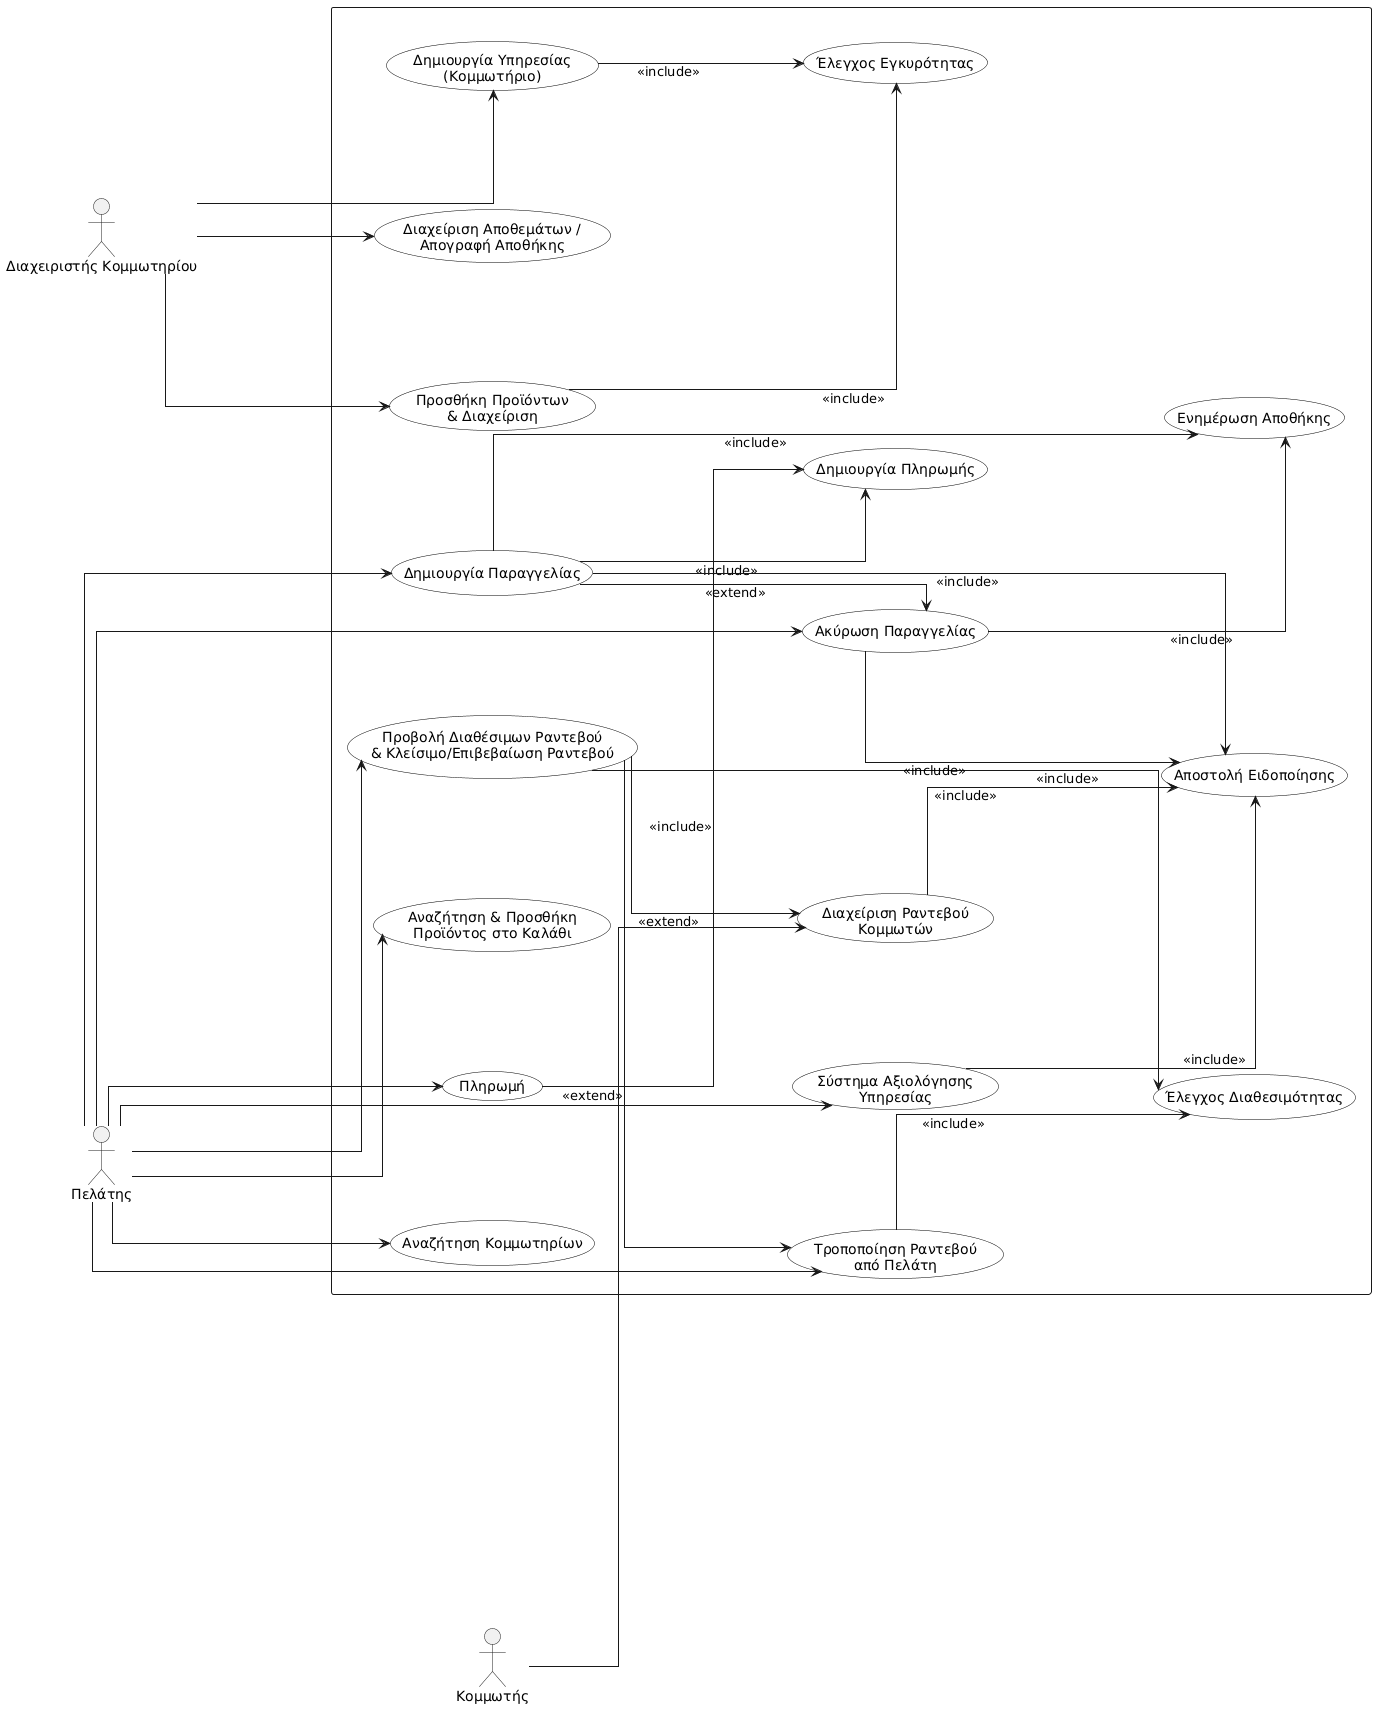
\includegraphics[width=0.8\textwidth]{usecase_d.PNG}
    \caption{Use-case διάγραμμα}
\end{figure}

\chapter{Domain-model-v0.1}
\section{Περιγραφή}
\begin{itemize}
    \item Χρήστης (User): Γενική υπερκλάση από την οποία κληρονομούν οι ρόλοι Customer, Hairdresser, SalonAdmin. Περιέχει τα βασικά στοιχεία σύνδεσης και ταυτοποίησης.
    \item Πελάτης (Customer): Χρήστης που μπορεί να κλείσει ραντεβού, να αγοράσει προϊόντα, να έχει καλάθι αγορών και ιστορικό παραγγελιών.
    \item Υπάλληλος (Employee): Χρήστης που εργάζεται στο κομμωτήριο, όπως κομμωτής ή διαχειριστής.
    \item Κομμωτής (Hairdresser): Χρήστης που παρέχει υπηρεσίες. Έχει πρόγραμμα διαθεσιμότητας και λίστα ραντεβού.
    \item Διαχειριστής (SalonAdmin): Χρήστης που διαχειρίζεται το κομμωτήριο, τους κομμωτές, τις υπηρεσίες και τα προϊόντα του ηλεκτρονικού καταστήματος.
    \item Κομμωτήριο (Salon): Οντότητα κομμωτηρίου με στοιχεία όπως όνομα, διεύθυνση, ώρες λειτουργίας και λίστες κομμωτών και υπηρεσιών.
    \item Υπηρεσία (Service): Παρεχόμενη υπηρεσία από το κομμωτήριο (π.χ. κούρεμα) με τίτλο, περιγραφή, διάρκεια και τιμή.
    \item Ραντεβού (Appointment): Ραντεβού μεταξύ πελάτη και κομμωτή για συγκεκριμένη υπηρεσία, με ημερομηνία, ώρα και κατάσταση.
    \item Πληρωμή (Payment): Πληρωμή για μια παραγγελία με ποσό, τρόπο πληρωμής, ημερομηνία και κατάσταση.
    \item Αξιολόγηση (Review): Αξιολόγηση από πελάτη για κομμωτήριο ή κομμωτή με βαθμολογία.
    \item Προϊόν (Product): Προϊόν προς πώληση στο ηλεκτρονικό κατάστημα, με όνομα, τιμή, απόθεμα και κατηγορία.
    \item Παραγγελία (Order): Παραγγελία πελάτη που περιλαμβάνει προϊόντα, συνολικό κόστος και κατάσταση αποστολής.
    \item Αποθήκη (Warehouse): Αποθήκη που διαχειρίζεται το απόθεμα των προϊόντων.
    \item Καλάθι (Cart): Καλάθι αγορών πελάτη που περιέχει προϊόντα και ποσότητες.
\end{itemize}
\clearpage
\section{Διάγραμμα}
Το παρακάτω διάγραμμα παρουσιάζει τις οντότητες του domain model και τις σχέσεις μεταξύ τους. Η σχεδίαση πραγματοποιήθηκε στο Draw.io, με τη συνεργασία και την επίβλεψη όλων των μελών της ομάδας.
\begin{figure}[H]
    \centering
    \includegraphics[width=1.0\textwidth]{domain-model.png}
    \caption{Domain Model}
\end{figure}

\chapter{Robustness-diagram-v1.0}
Παρακάτω παρατίθονται τα διαγράμματα ευρωστίας για την εφαρμογή BeautyHub με βάση την σειρά που εμφανίζονται και οι περιπτώσεις χρήσης. Χρησιμοποιήθηκε το εργαλείο drawio για την σχεδίαση των διαγραμμάτων, με την βοήθεια και επίβλεψη όλων των μελών της ομάδας.

\section{Αναζήτηση Κομμωτηρίων}
\begin{figure}[H]
    \centering
    
\includegraphics[width=1.0\textwidth]{UCS/UC1.png}
    \caption{Robustness diagram για την περίπτωση χρήσης "Αναζήτηση Κομμωτηρίων"}
\end{figure}
\clearpage
\section{Προβολή Διαθέσιμων Ραντεβού & Κλείσιμο Ραντεβού}
\vfill
\begin{figure}[H]
    \centering
    
\includegraphics[width=1.0\textwidth]{UCS/UC2.png}
    \caption{Robustness diagram για την περίπτωση χρήσης "Προβολή Διαθέσιμων Ραντεβού & Κλείσιμο Ραντεβού"}
\end{figure}
\vfill
\clearpage
\section{Διαχείριση Ραντεβού Κομμωτών}
\vfill
\begin{figure}[H]
    \centering
    
\includegraphics[width=1.0\textwidth]{UCS/UC3.png}
    \caption{Robustness diagram για την περίπτωση χρήσης "Διαχείριση Ραντεβού Κομμωτών"}
\end{figure}
\vfill
\clearpage
\section{Διαχείριση Αποθεμάτων}
\vfill
\begin{figure}[H]
    \centering
    
\includegraphics[width=1.0\textwidth]{UCS/UC4.png}
    \caption{Robustness diagram για την περίπτωση χρήσης "Διαχείριση Αποθεμάτων"}
\end{figure}
\vfill
\clearpage
\section{Πληρωμή}
\vfill
\begin{figure}[H]
    \centering
    
\includegraphics[width=1.0\textwidth]{UCS/UC5.png}
    \caption{Robustness diagram για την περίπτωση χρήσης "Πληρωμή "}
\end{figure}
\vfill
\clearpage
\section{Σύστημα Αξιολόγησης Υπηρεσίας}
\vfill
\begin{figure}[H]
    \centering
    
\includegraphics[width=1.0\textwidth]{UCS/UC6.png}
    \caption{Robustness diagram για την περίπτωση χρήσης "Σύστημα Αξιολόγησης Υπηρεσίας "}
\end{figure}.
\vfill
\clearpage
\section{Δημιουργία Υπηρεσίας από το Κομμωτήριο}
\vfill
\begin{figure}[H]
    \centering
    
\includegraphics[width=1.0\textwidth]{UCS/UC7.png}
    \caption{Robustness diagram για την περίπτωση χρήσης "Δημιουργία Υπηρεσίας από το Κομμωτήριο"}
\end{figure}
\vfill
\clearpage
\section{Προσθήκη Προϊόντων & Διαχείριση}
\vfill
\begin{figure}[H]
    \centering
    
\includegraphics[width=1.0\textwidth]{UCS/UC8.png}
    \caption{Robustness diagram για την περίπτωση χρήσης "Προσθήκη Προϊόντων & Διαχείριση"}
\end{figure}
\vfill
\clearpage
\section{Δημιουργία Παραγγελίας}
\vfill
\begin{figure}[H]
    \centering
    
\includegraphics[width=1.0\textwidth]{UCS/UC9.png}
    \caption{Robustness diagram για την περίπτωση χρήσης "Δημιουργία Παραγγελίας"}
\end{figure}
\vfill
\clearpage
\section{Ακύρωση Παραγγελίας}
\vfill
\begin{figure}[H]
    \centering
    
\includegraphics[width=1.0\textwidth]{UCS/UC10.png}
    \caption{Robustness diagram για την περίπτωση χρήσης "Ακύρωση Παραγγελίας"}
\end{figure}
\vfill
\clearpage
\section{Αναζήτηση και προσθήκη προϊόντος στο καλάθι}
\vfill
\begin{figure}[H]
    \centering
    
\includegraphics[width=1.0\textwidth]{UCS/UC11.png}
    \caption{Robustness diagram για την περίπτωση χρήσης "Αναζήτηση και προσθήκη προϊόντος στο καλάθι"}
\end{figure}
\vfill
\clearpage
\section{Τροποποίηση ραντεβού από πελάτη}
\vfill
\begin{figure}[H]
    \centering
    
\includegraphics[width=1.0\textwidth]{UCS/UC12.png}
    \caption{Robustness diagram για την περίπτωση χρήσης "Τροποποίηση ραντεβού από πελάτη"}
\end{figure}
\vfill



\chapter{Sequence-diagram-v1.0}
Παρακάτω παρατίθονται τα διαγράμματα ακολουθίας για την εφαρμογή BeautyHub με βάση την σειρά που εμφανίζονται και οι περιπτώσεις χρήσης. Χρησιμοποιήθηκε το εργαλείο drawio για την σχεδίαση των διαγραμμάτων, με την βοήθεια και επίβλεψη όλων των μελών της ομάδας.


\section{Αναζήτηση Κομμωτηρίων}
\begin{figure}[H]
    \centering
    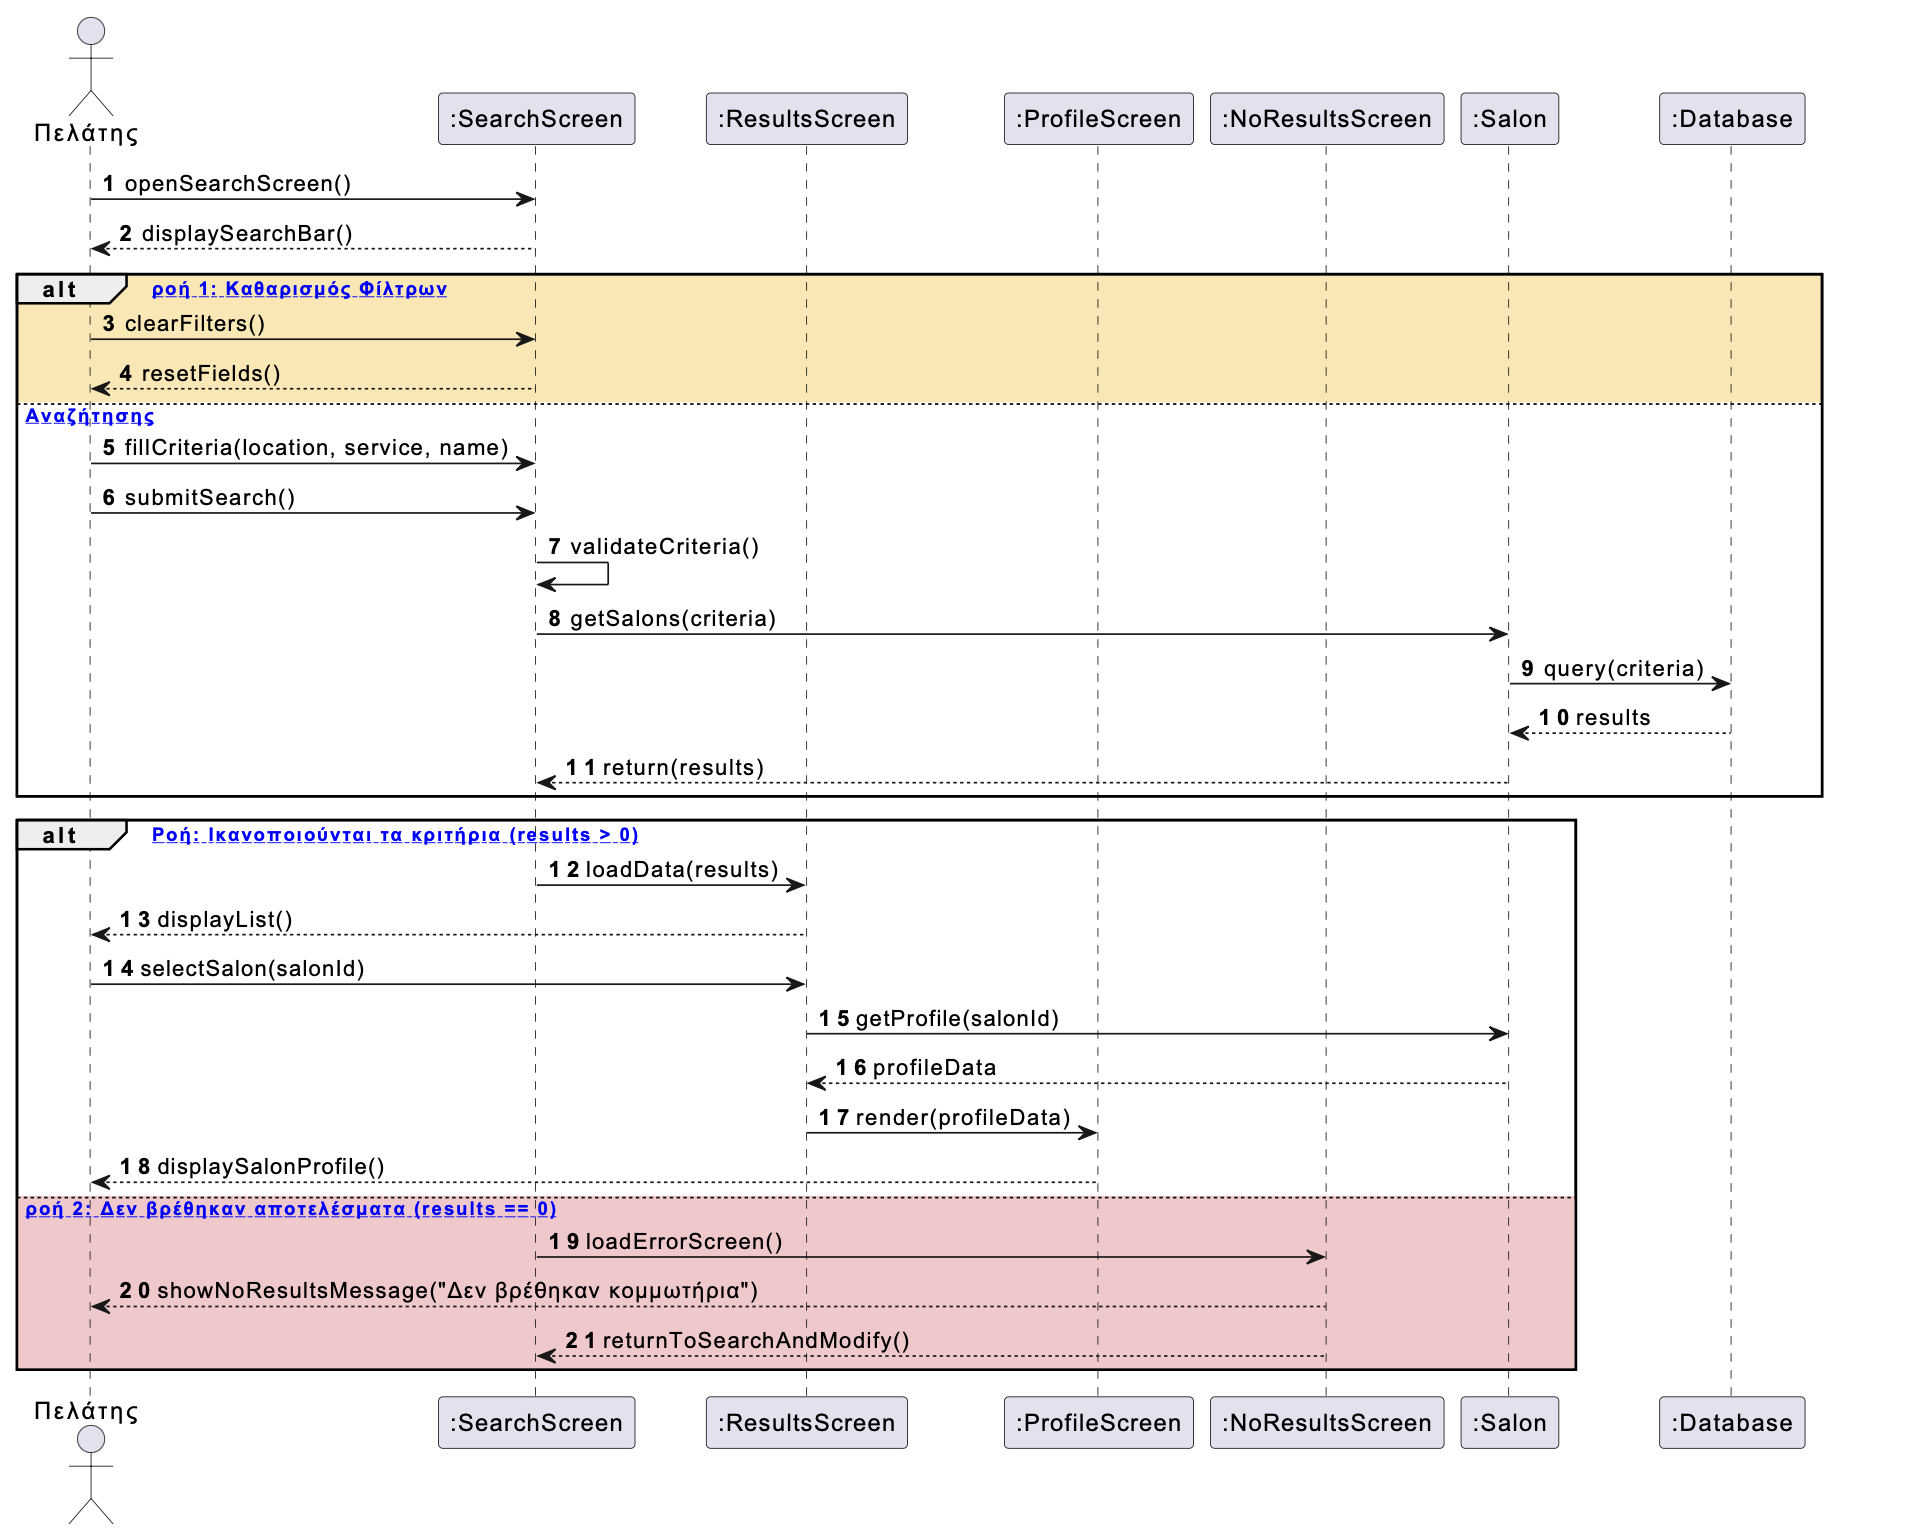
\includegraphics[width=1.0\textwidth]{../sequence diagrams/sd1.png}
    \caption{Sequence diagram για την περίπτωση χρήσης "Αναζήτηση Κομμωτηρίων"}
\end{figure}
\vfill
\clearpage
\section{Προβολή Διαθέσιμων Ραντεβού \& Κλείσιμο Ραντεβού}
\vfill
\begin{figure}[H]
    \centering
    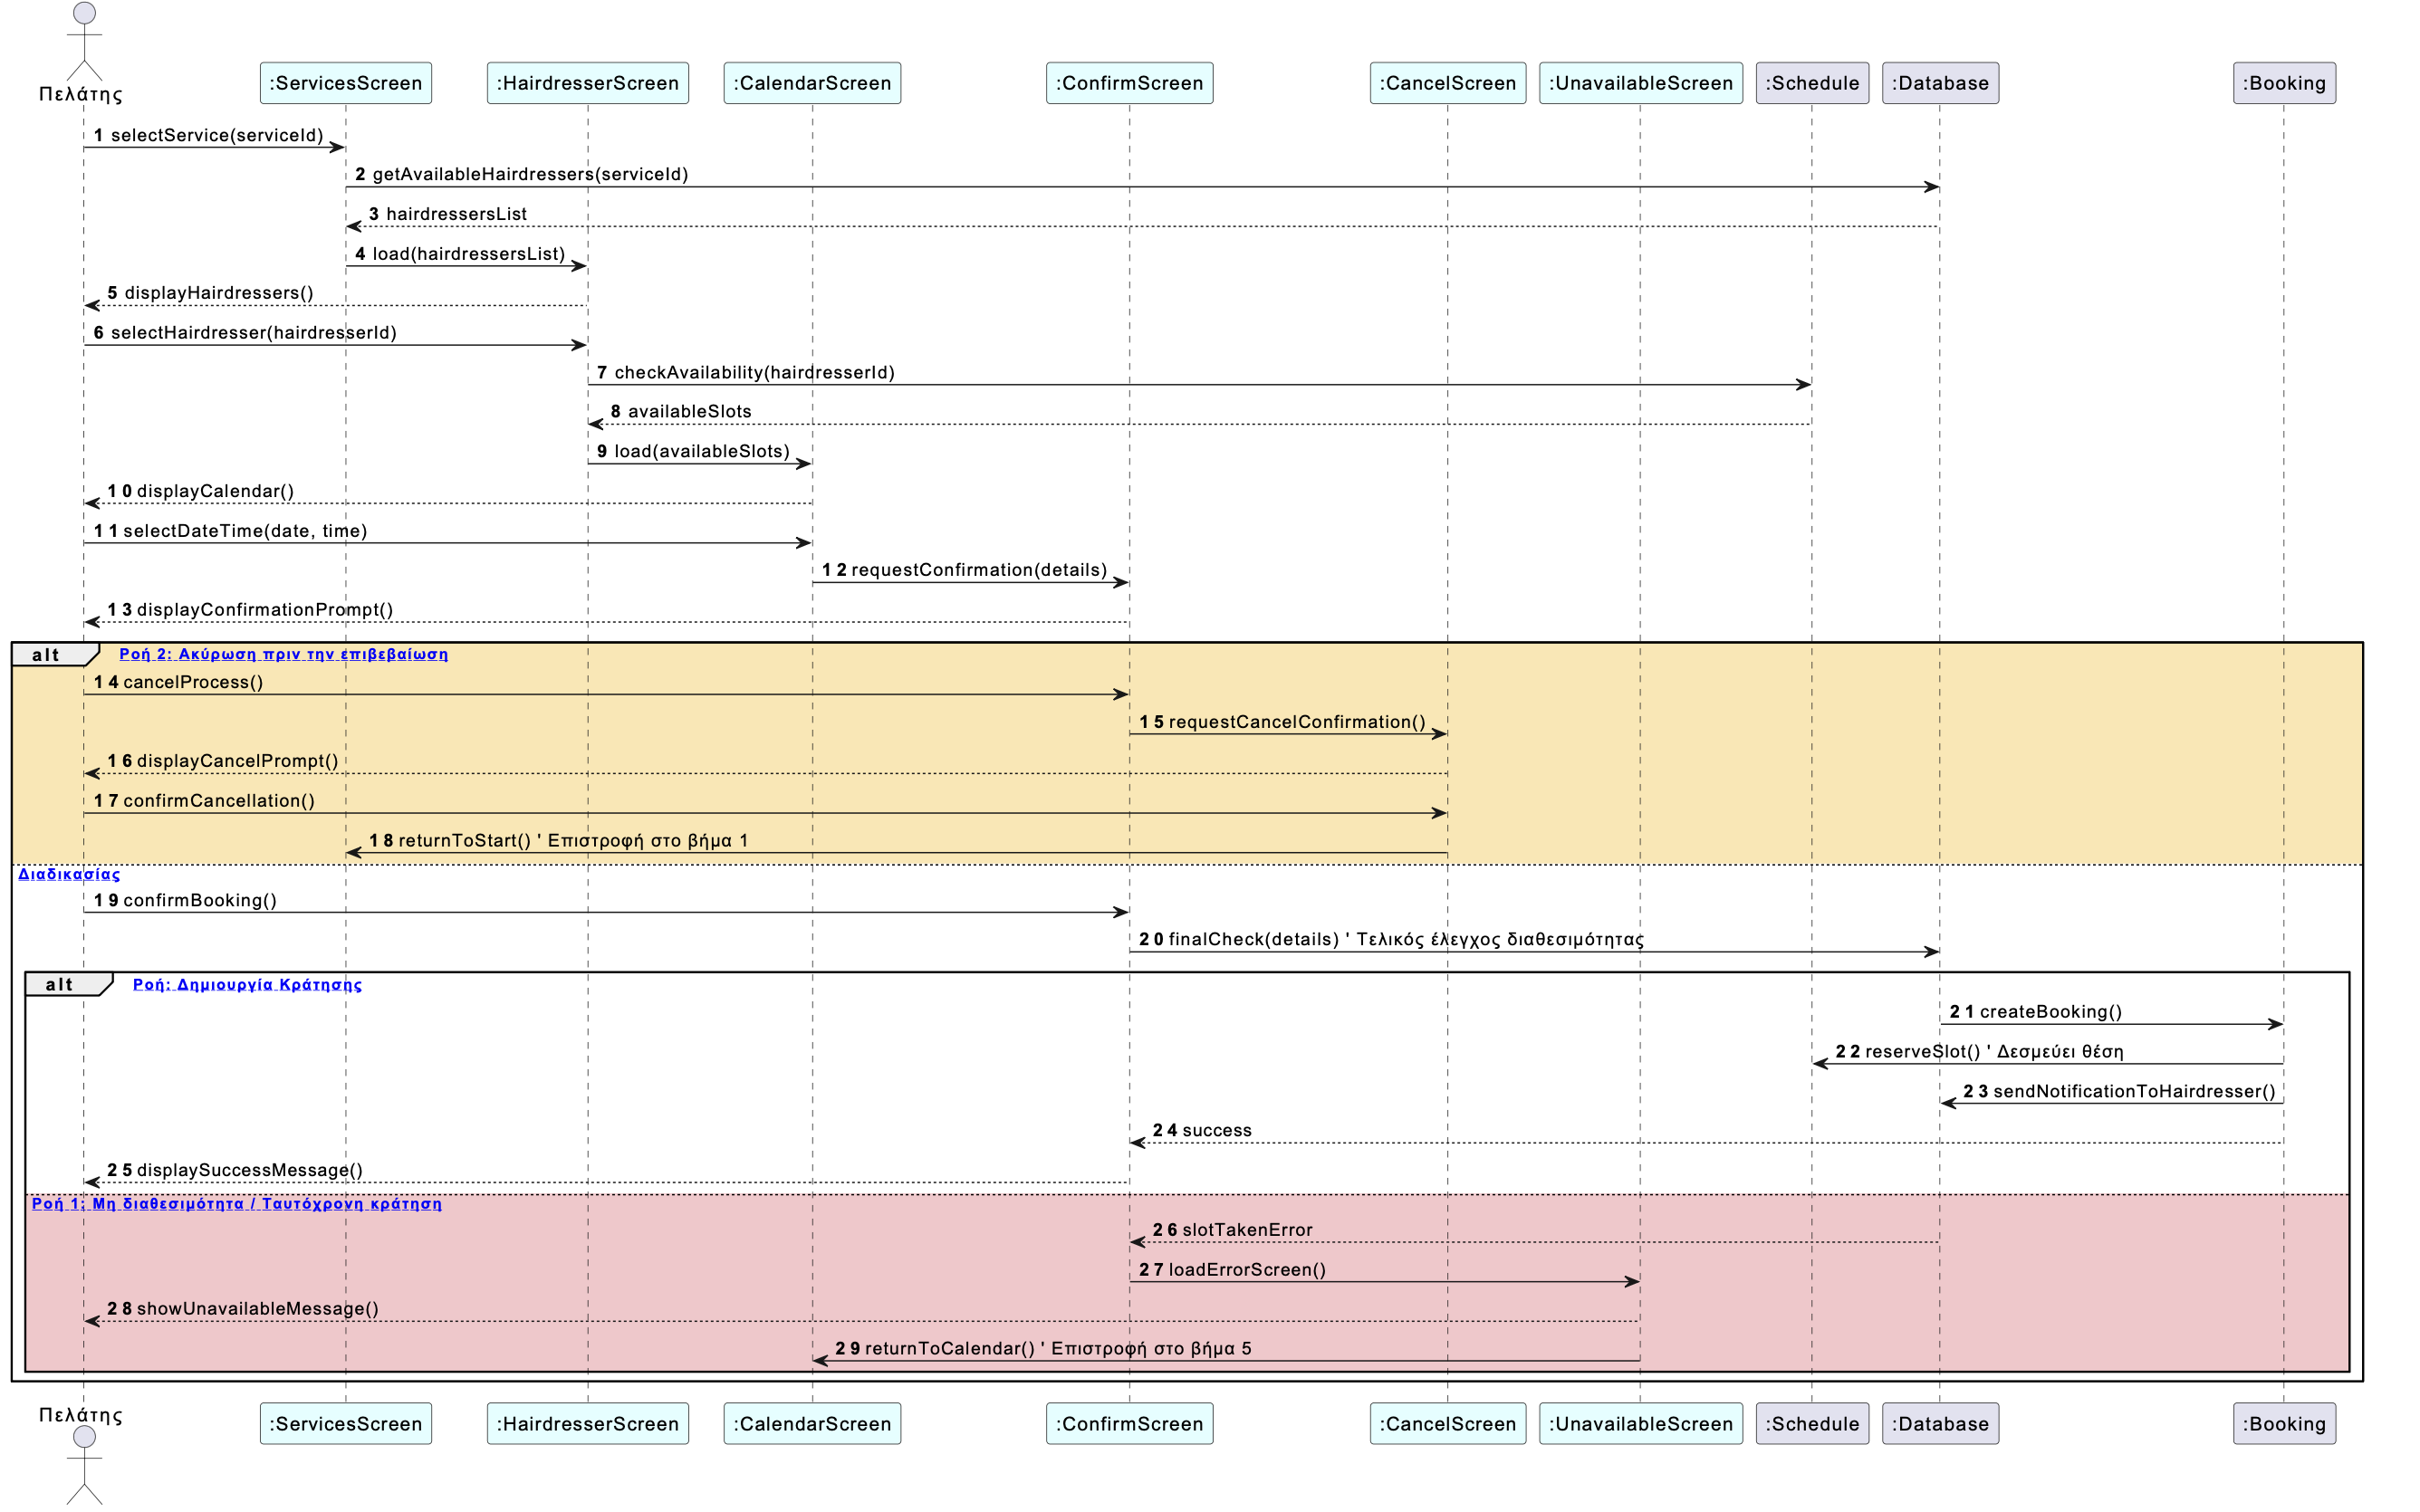
\includegraphics[width=1.0\textwidth]{../sequence diagrams/sd2.png}
    \caption{Sequence diagram για την περίπτωση χρήσης "Προβολή Διαθέσιμων Ραντεβού \& Κλείσιμο Ραντεβού"}
\end{figure}
\vfill
\clearpage
\section{Διαχείριση Ραντεβού Κομμωτών}
\vfill
\begin{figure}[H]
    \centering
    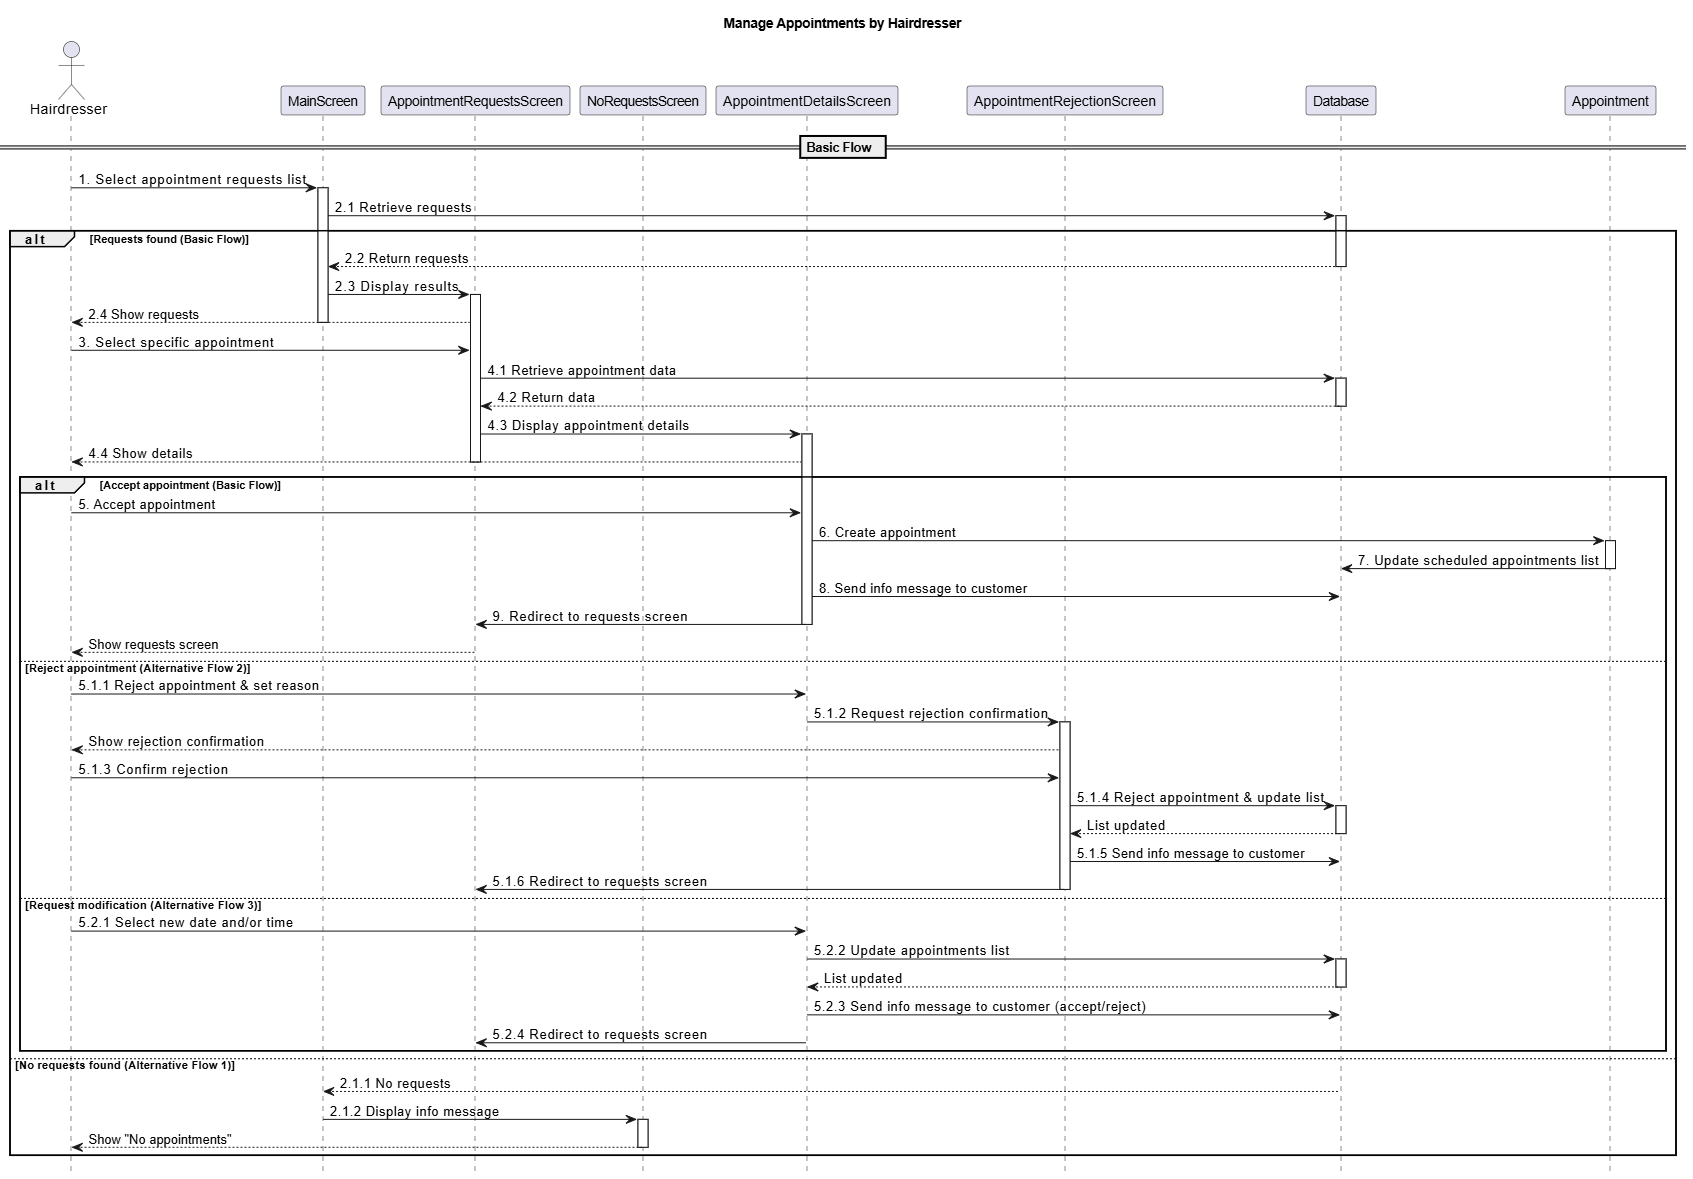
\includegraphics[width=1.0\textwidth]{../sequence diagrams/sd3.png}
    \caption{Sequence diagram για την περίπτωση χρήσης "Διαχείριση Ραντεβού Κομμωτών"}
\end{figure}
\vfill
\clearpage
\section{Διαχείριση Αποθεμάτων}
\vfill
\begin{figure}[H]
    \centering
    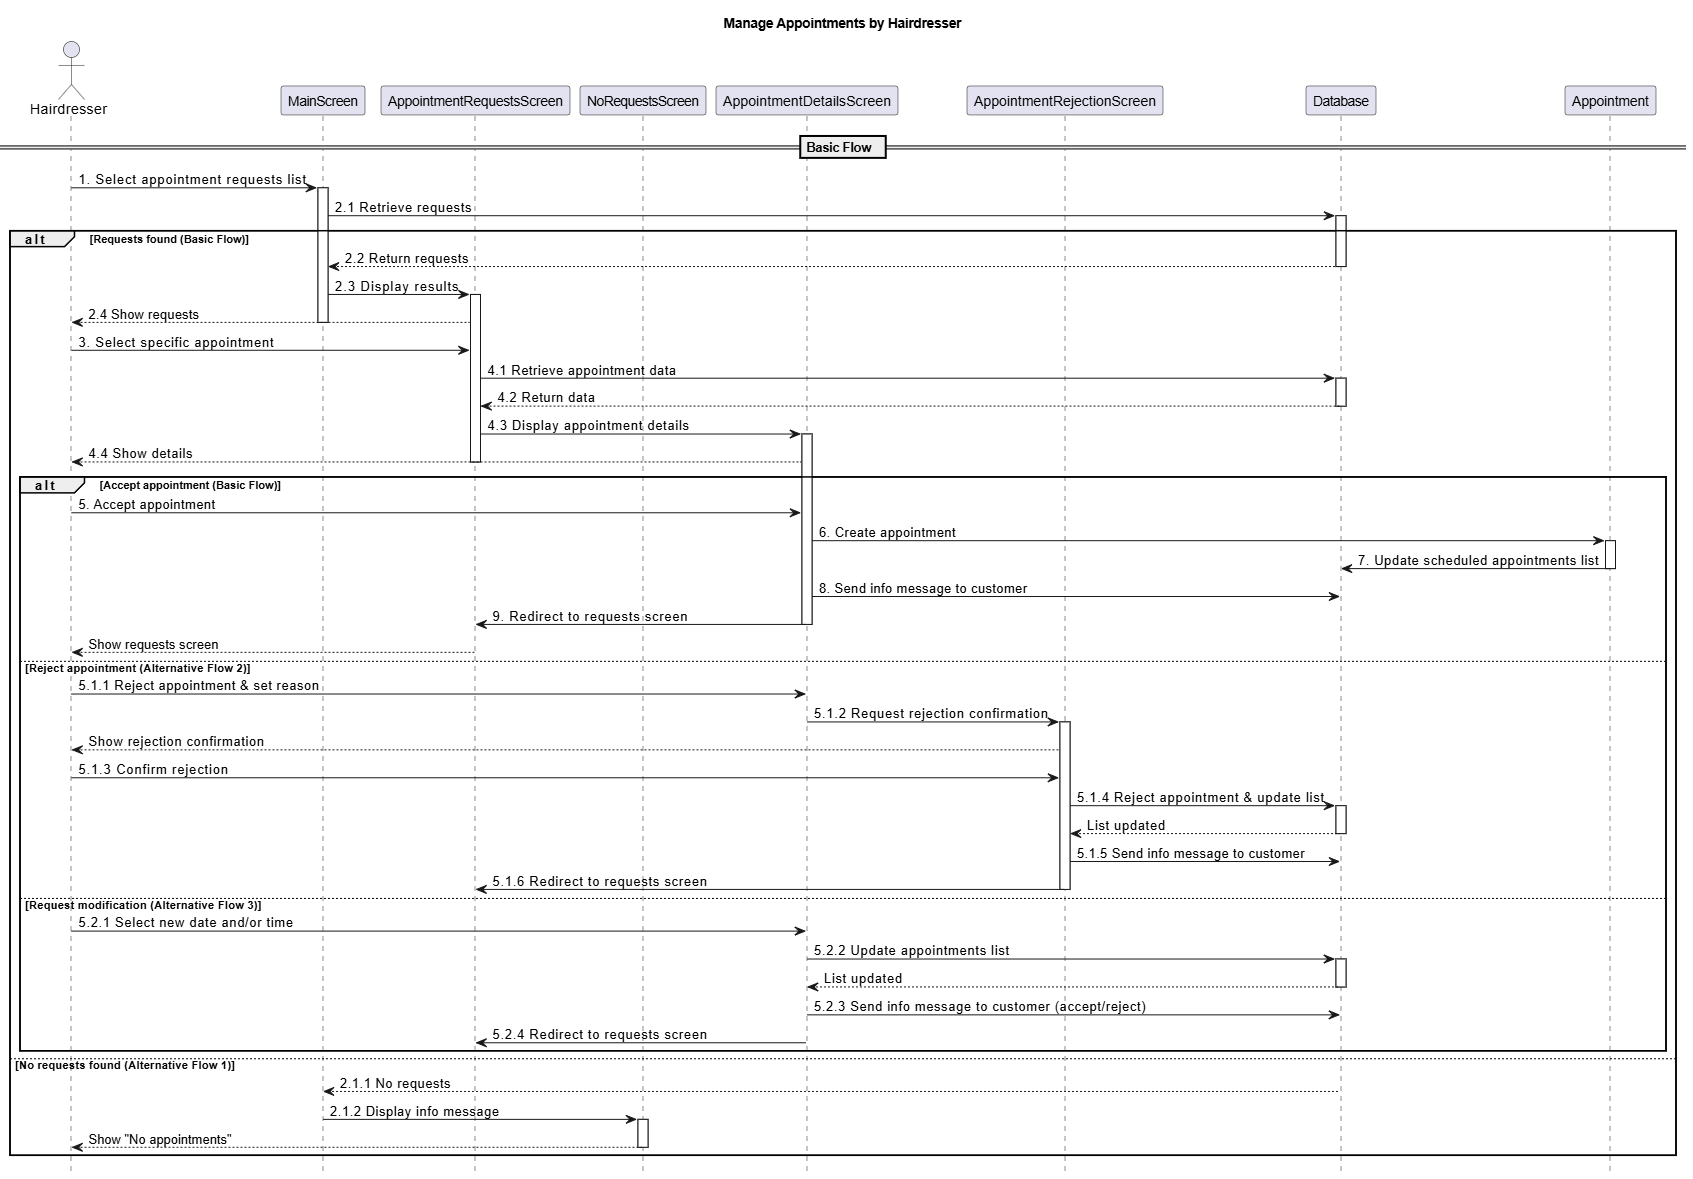
\includegraphics[width=1.0\textwidth]{../sequence diagrams/sd4.png}
    \caption{Sequence diagram για την περίπτωση χρήσης "Διαχείριση Αποθεμάτων"}
\end{figure}
\vfill
\clearpage
\section{Πληρωμή}
\begin{figure}[H]
    \centering
    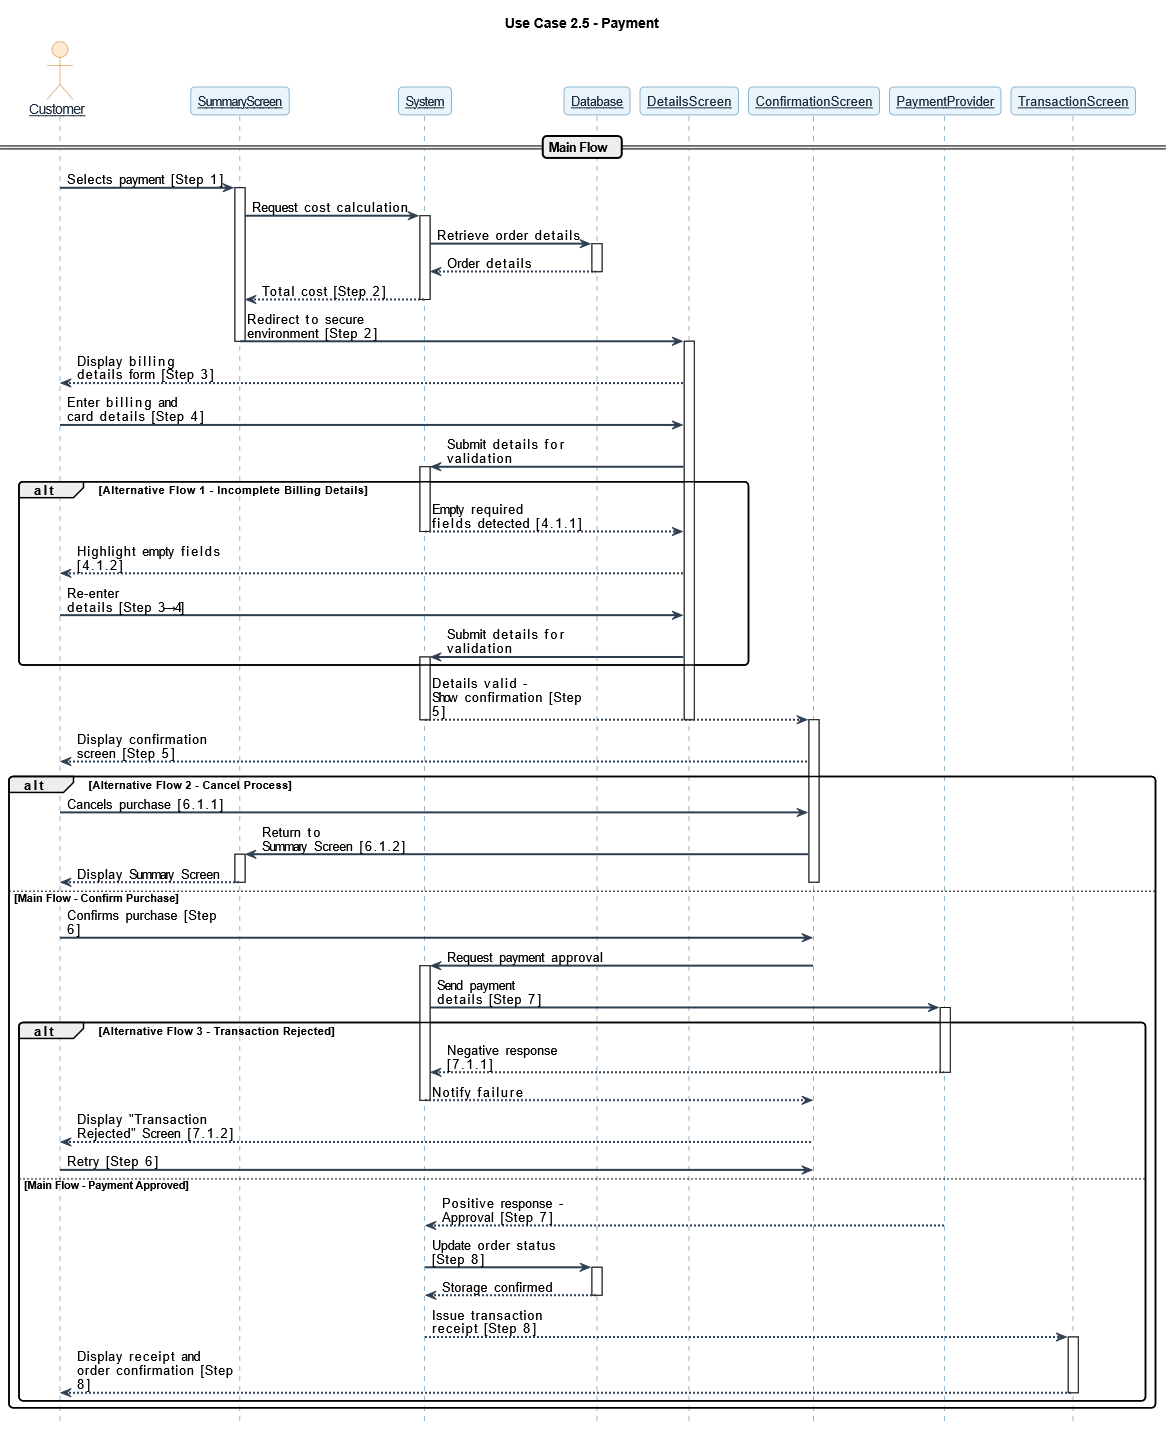
\includegraphics[width=1.0\textwidth]{../sequence diagrams/SD5.png}
    \caption{Sequence diagram για την περίπτωση χρήσης "Πληρωμή"}
\end{figure}
\vfill
\section{Σύστημα Αξιολόγησης Υπηρεσίας}
\vfill
\begin{figure}[H]
    \centering
    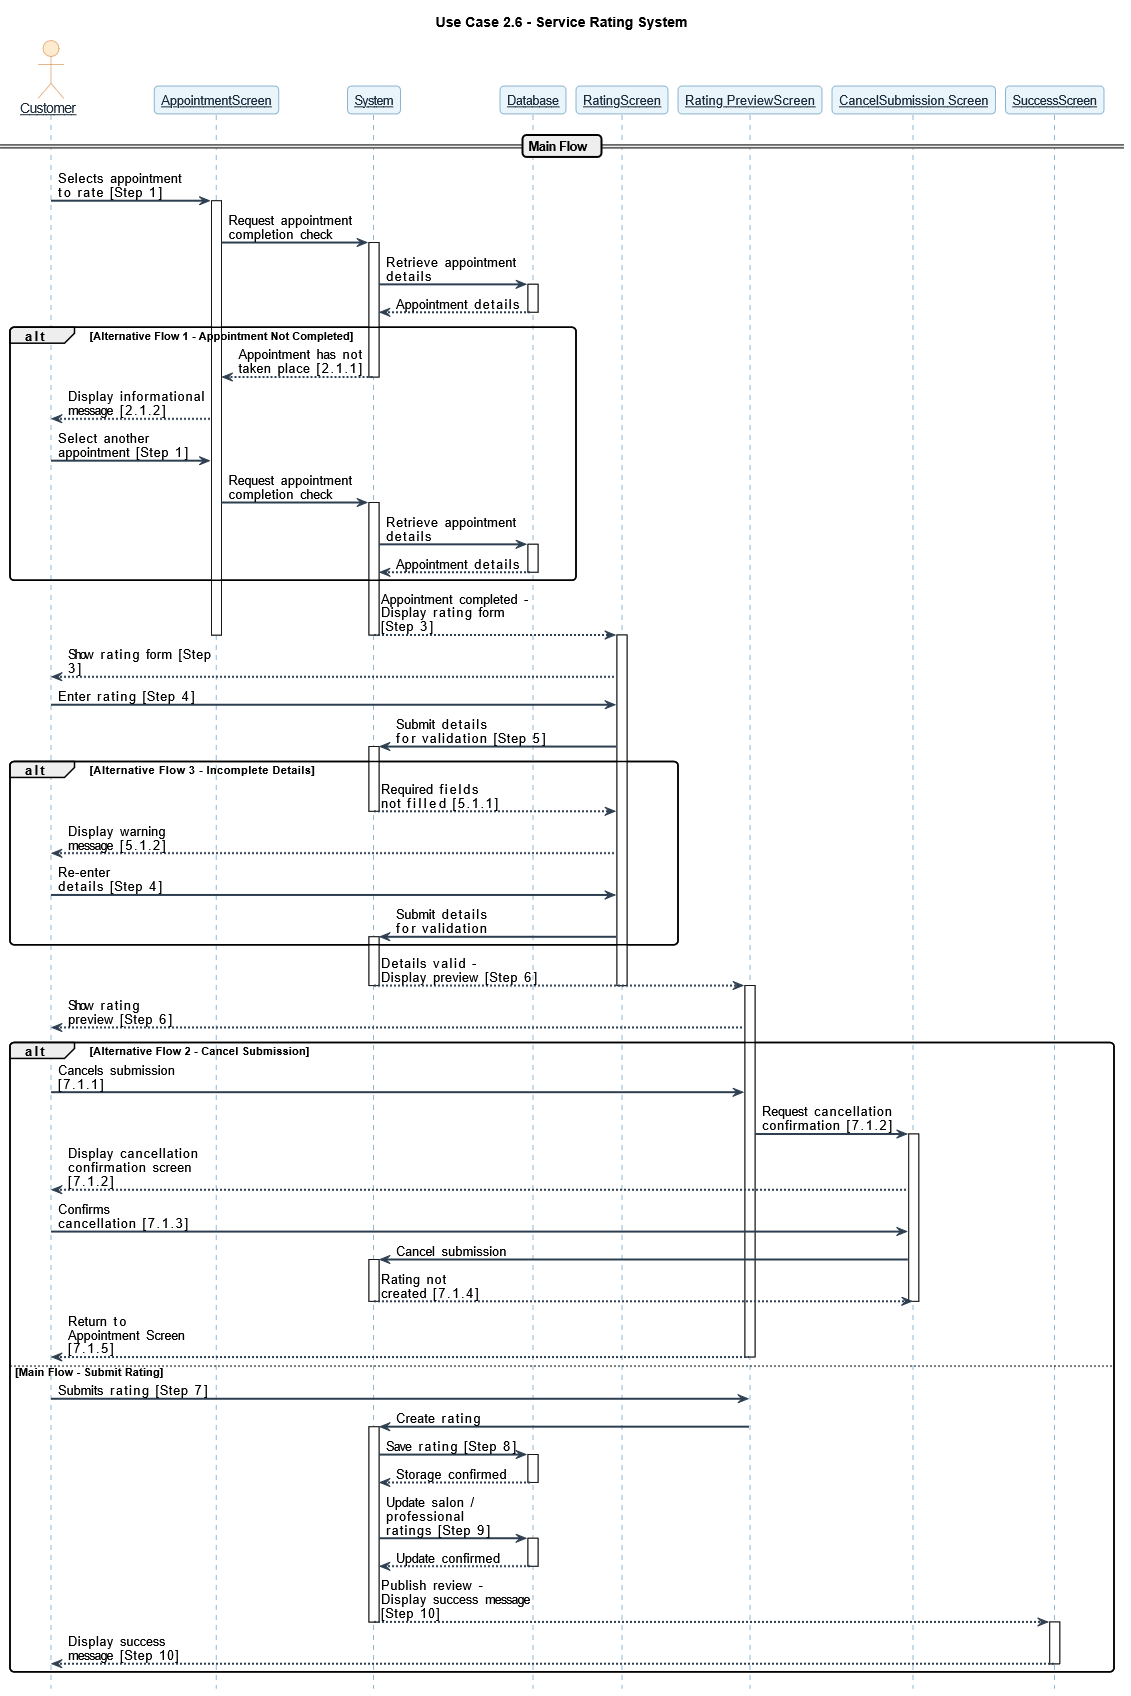
\includegraphics[width=0.9\textwidth]{../sequence diagrams/SD6.png}
    \caption{Sequence diagram για την περίπτωση χρήσης "Σύστημα Αξιολόγησης Υπηρεσίας"}
\end{figure}
\vfill
\clearpage
\section{Δημιουργία Υπηρεσίας από το Κομμωτήριο}
\vfill
\begin{figure}[H]
    \centering
    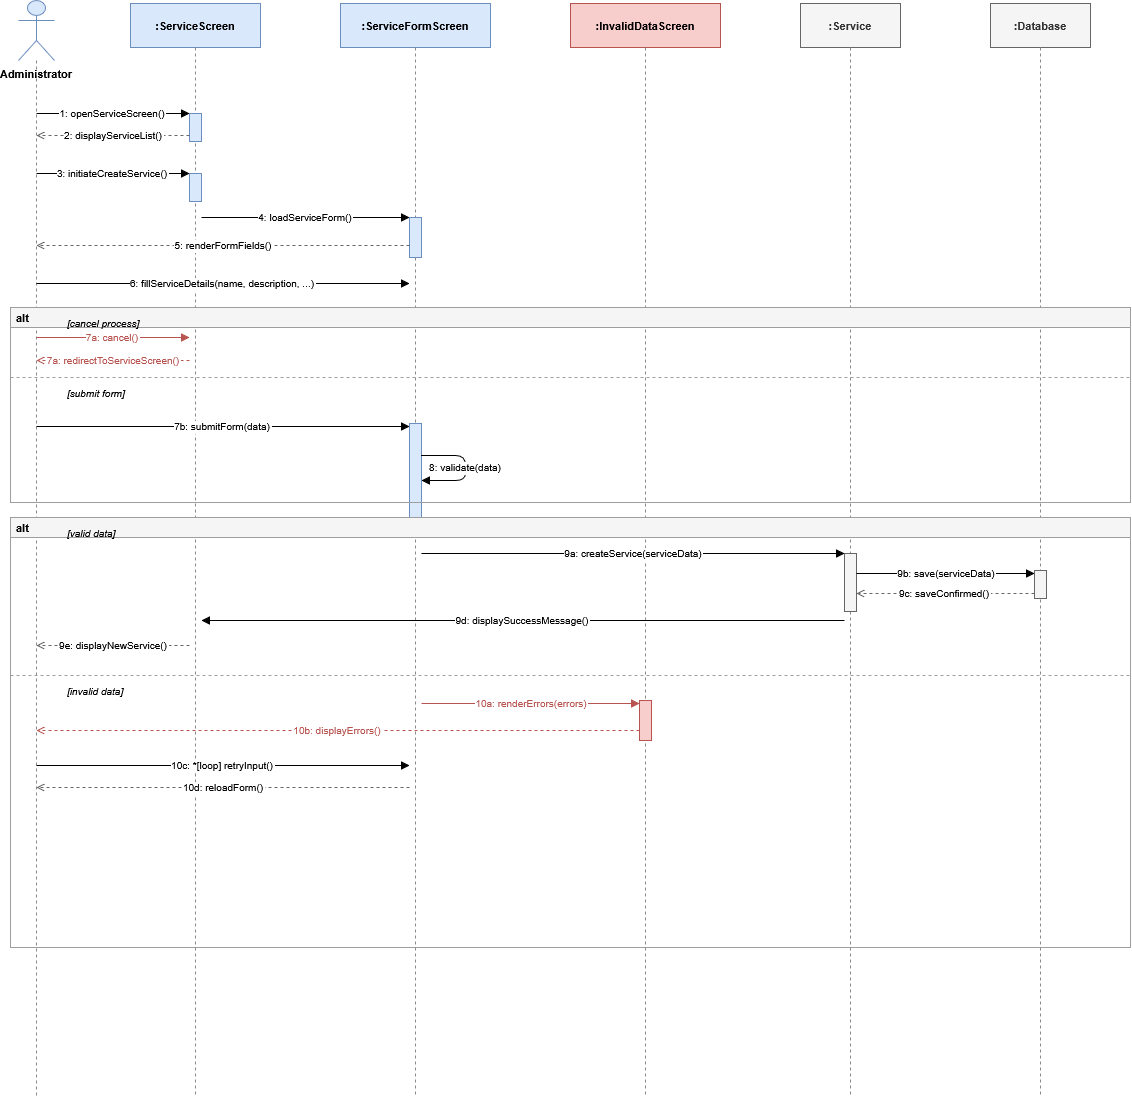
\includegraphics[width=1.0\textwidth]{../sequence diagrams/SD7.png}
    \caption{Sequence diagram για την περίπτωση χρήσης "Δημιουργία Υπηρεσίας από το Κομμωτήριο"}
\end{figure}
\vfill
\clearpage
\section{Προσθήκη Προϊόντων \& Διαχείριση}
\vfill
\begin{figure}[H]
    \centering
    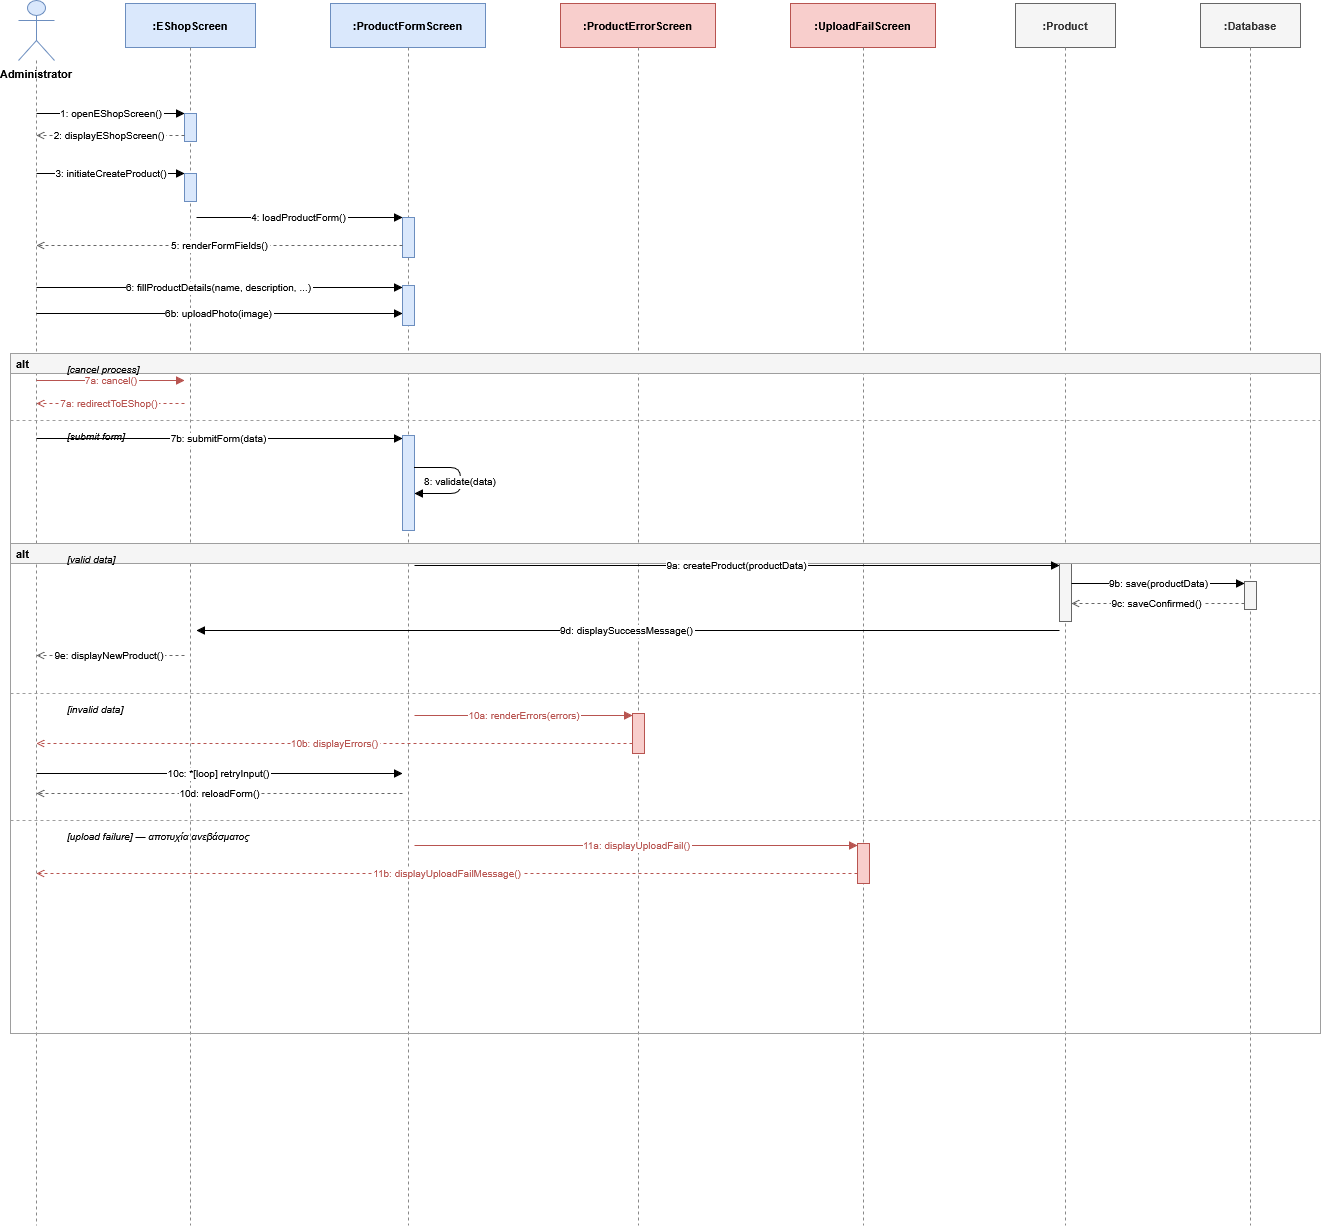
\includegraphics[width=1.0\textwidth]{../sequence diagrams/SD8.png}
    \caption{Sequence diagram για την περίπτωση χρήσης "Προσθήκη Προϊόντων \& Διαχείριση"}
\end{figure}
\vfill
\clearpage
\section{Δημιουργία Παραγγελίας}
\vfill
\begin{figure}[H]
    \centering
    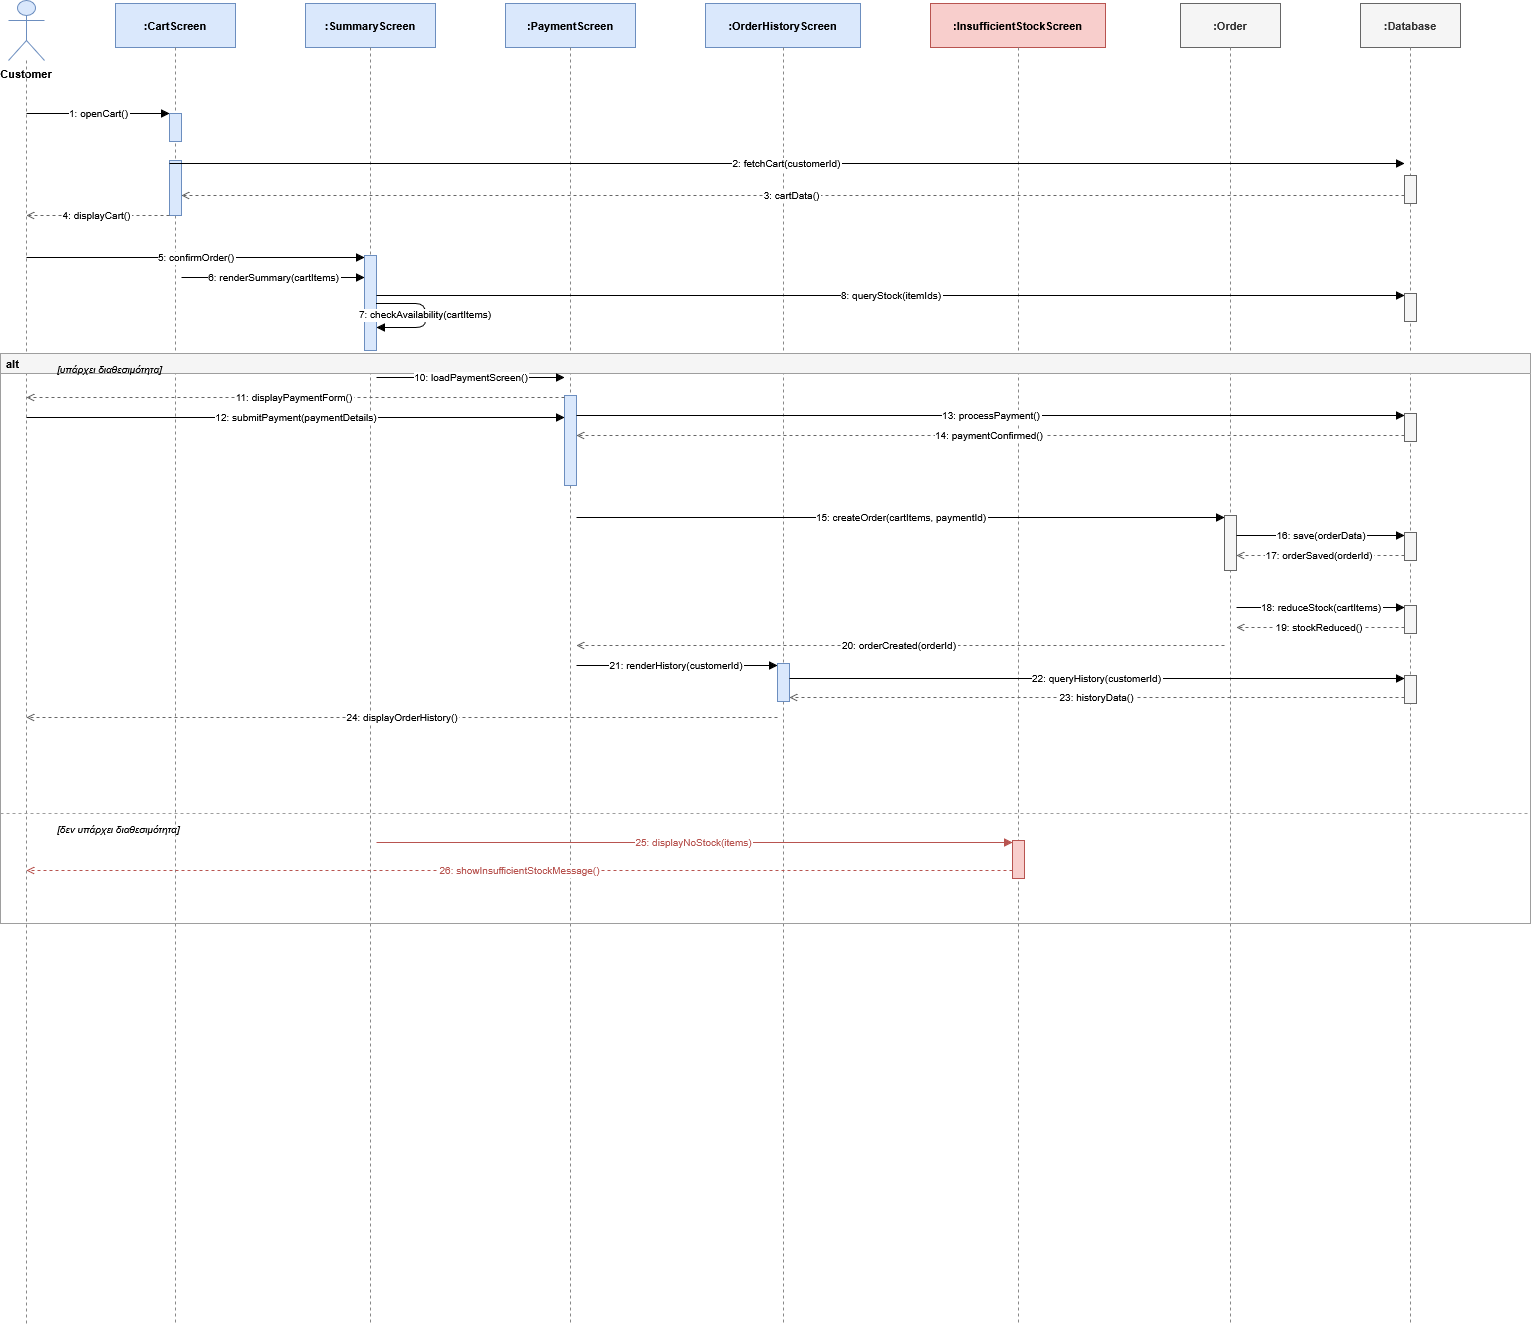
\includegraphics[width=1.0\textwidth]{../sequence diagrams/SD9.png}
    \caption{Sequence diagram για την περίπτωση χρήσης "Δημιουργία Παραγγελίας"}
\end{figure}
\vfill
\clearpage
\section{Ακύρωση Παραγγελίας}
\vfill
\begin{figure}[H]
    \centering
    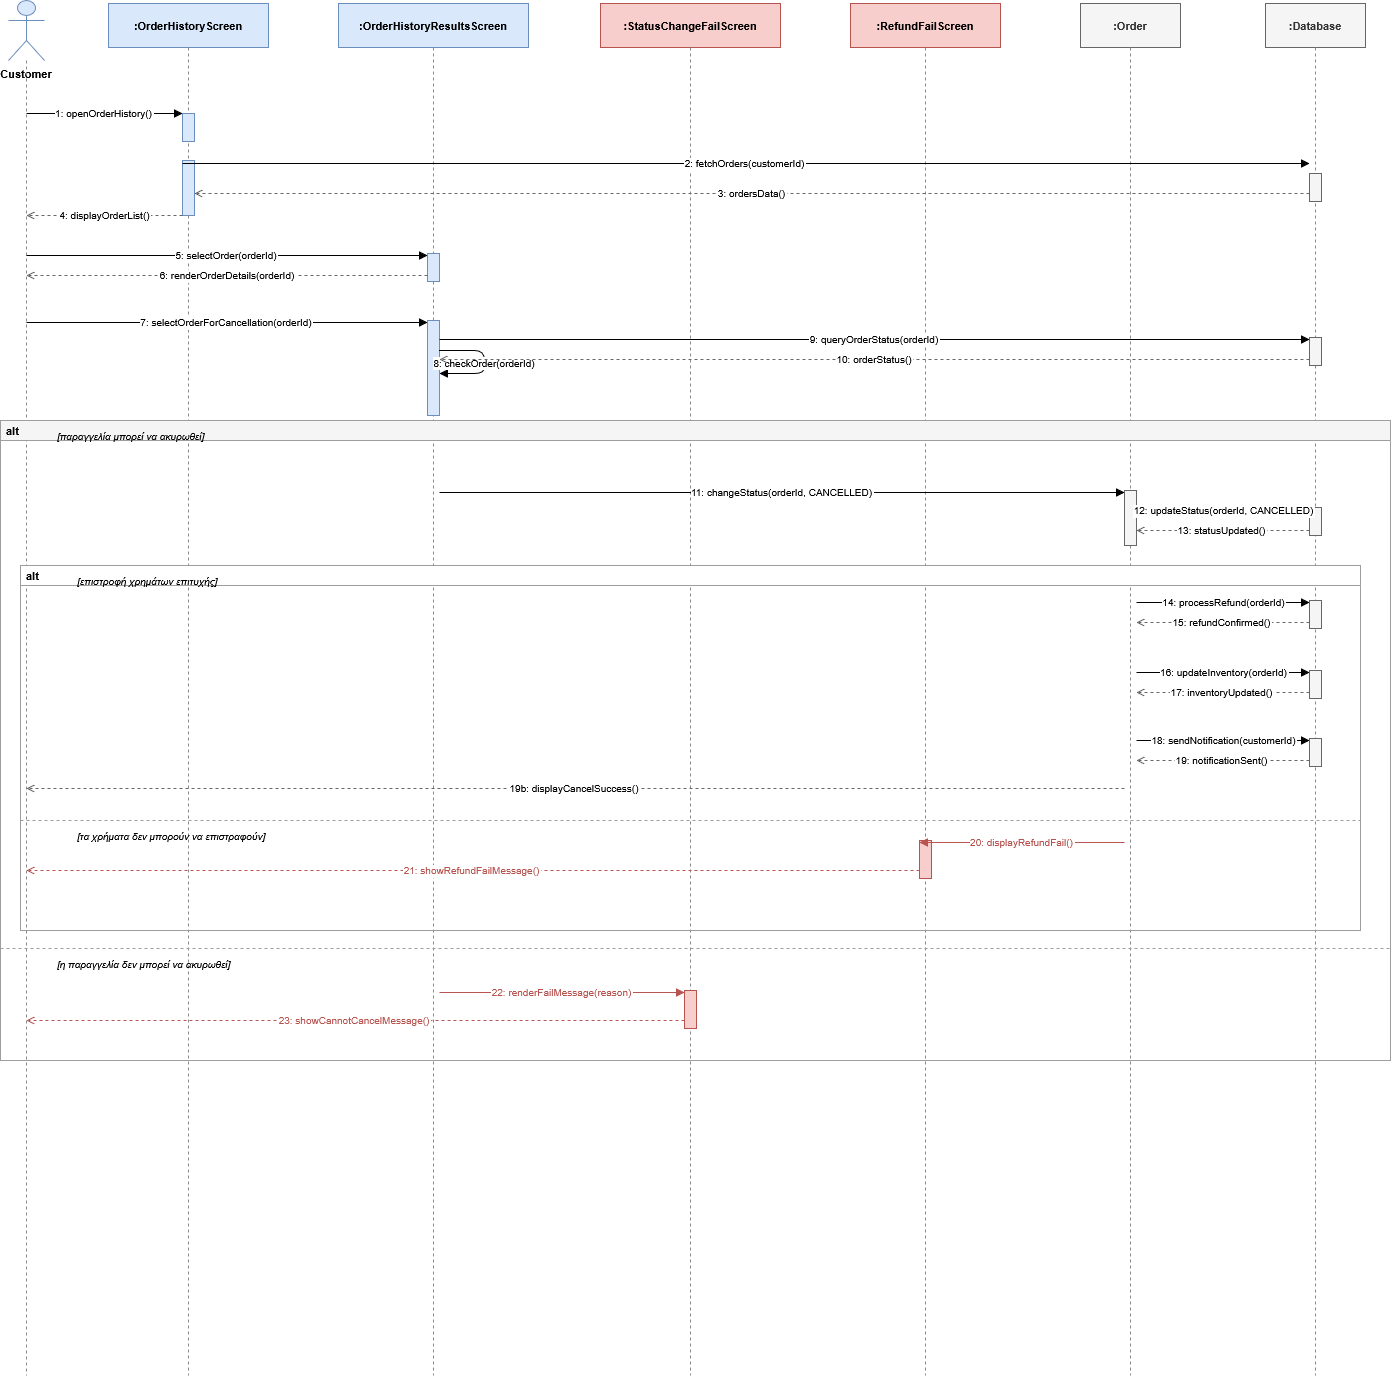
\includegraphics[width=1.0\textwidth]{../sequence diagrams/SD10.png}
    \caption{Sequence diagram για την περίπτωση χρήσης "Ακύρωση Παραγγελίας"}
\end{figure}
\vfill
\clearpage
\section{Αναζήτηση και προσθήκη προϊόντος στο καλάθι}
\vfill
\begin{figure}[H]
    \centering
    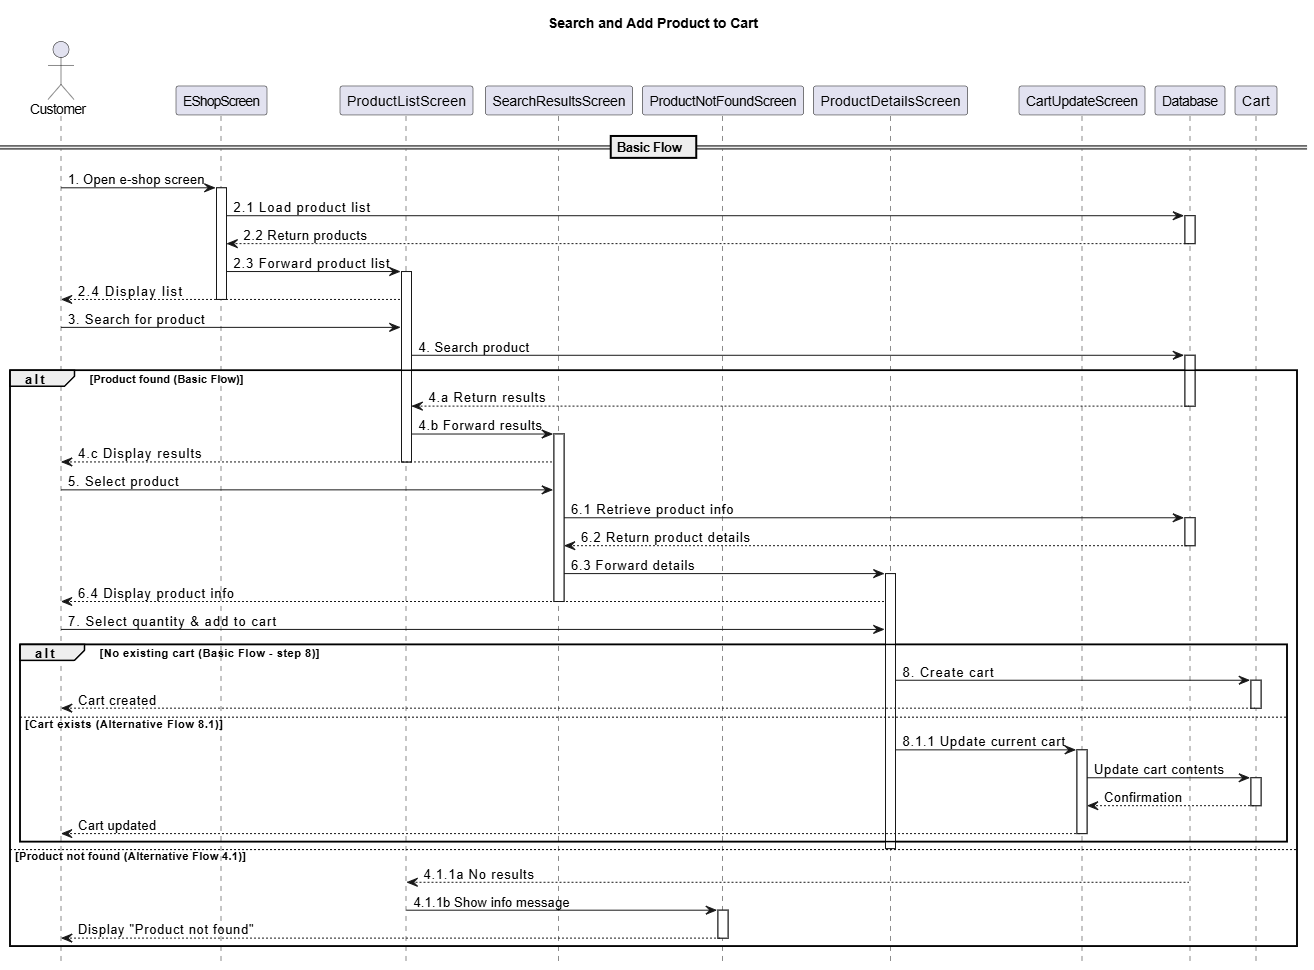
\includegraphics[width=1.0\textwidth]{../sequence diagrams/sd11.png}
    \caption{Sequence diagram για την περίπτωση χρήσης "Αναζήτηση και προσθήκη προϊόντος στο καλάθι"}
\end{figure}
\vfill
\clearpage
\section{Τροποποίηση ραντεβού από πελάτη}
\vfill
\begin{figure}[H]
    \centering
    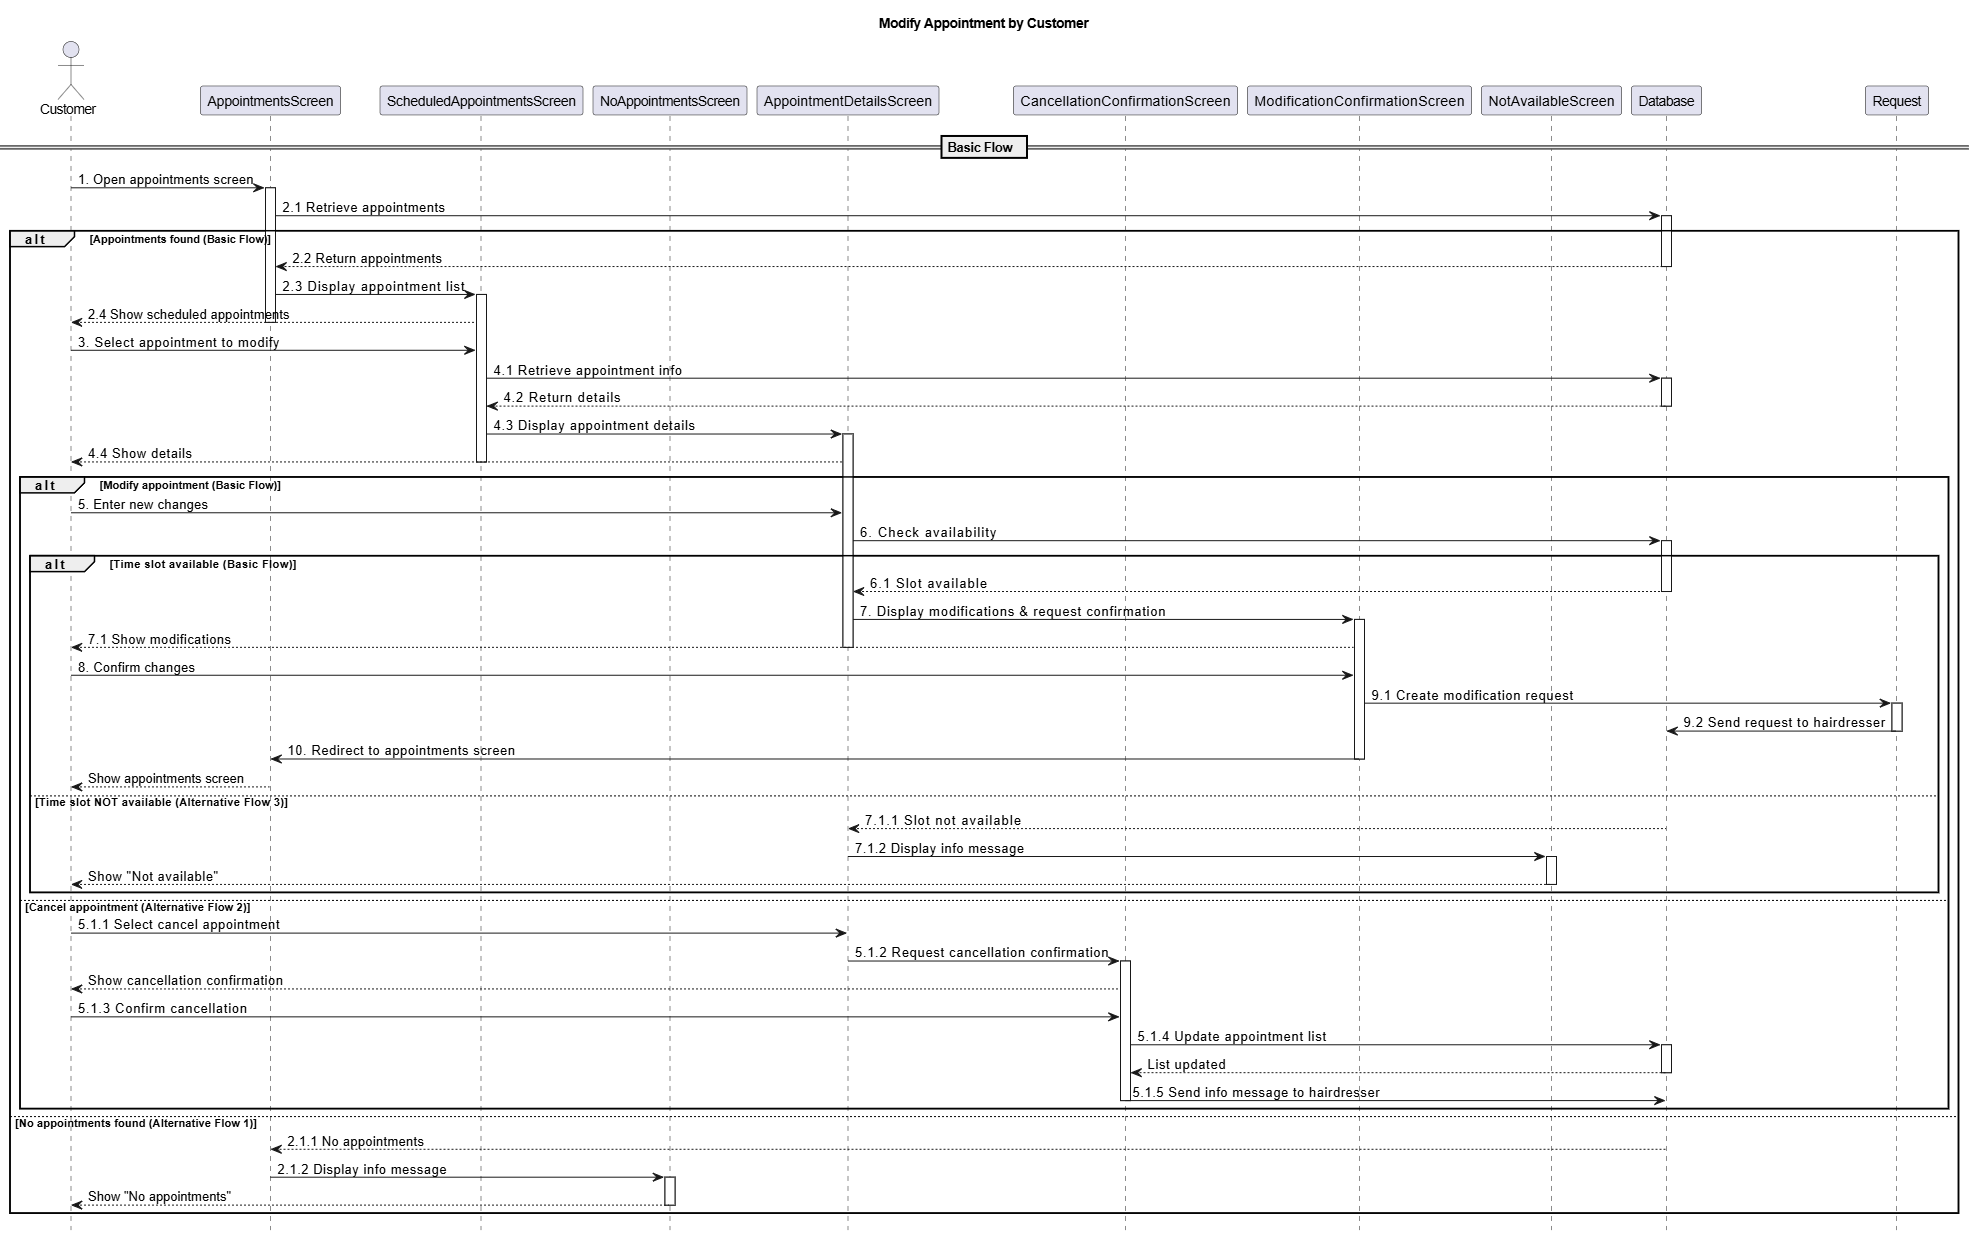
\includegraphics[width=1.0\textwidth]{../sequence diagrams/sd12.png}
    \caption{Sequence diagram για την περίπτωση χρήσης "Τροποποίηση ραντεβού από πελάτη"}
\end{figure}
\vfill

\end{document}